\documentclass[11pt,a4paper,openany]{book}
\usepackage[T1]{fontenc}
\usepackage[utf8]{inputenc}
\usepackage{lmodern,textcomp}
\usepackage[margin=2.2cm]{geometry}
\usepackage{graphicx,float,booktabs,tabularx,amsmath,amssymb,xcolor,enumitem}
\usepackage[most]{tcolorbox}
\usepackage[hidelinks]{hyperref}
\usepackage{microtype}
\graphicspath{{./}}
\definecolor{accent}{HTML}{FF5722}
\hypersetup{pdftitle={AnaTele Illustrated Guide: learn drone flight-log investigation from scratch},
  pdfauthor={Avinash Chandra Gupta},
  pdfsubject={ArduPilot flight log analysis, drone crash investigation},
  pdfkeywords={AnaTele, Avinash Chandra Gupta, Avinash Gupta, ArduPilot, MAVLink, drone, crash investigation, flight log, tutorial}}
\newtcolorbox{guidebox}[2]{enhanced,breakable,colback=#2!5!white,colframe=#2,fonttitle=\bfseries,title={#1},
  boxrule=0.6pt,arc=2pt,left=6pt,right=6pt}
\setlist{itemsep=2pt}
\setlength{\parskip}{0.5em}
\setlength{\parindent}{0pt}
\emergencystretch=2em
\begin{document}
\begin{titlepage}
\centering
\vspace*{2cm}
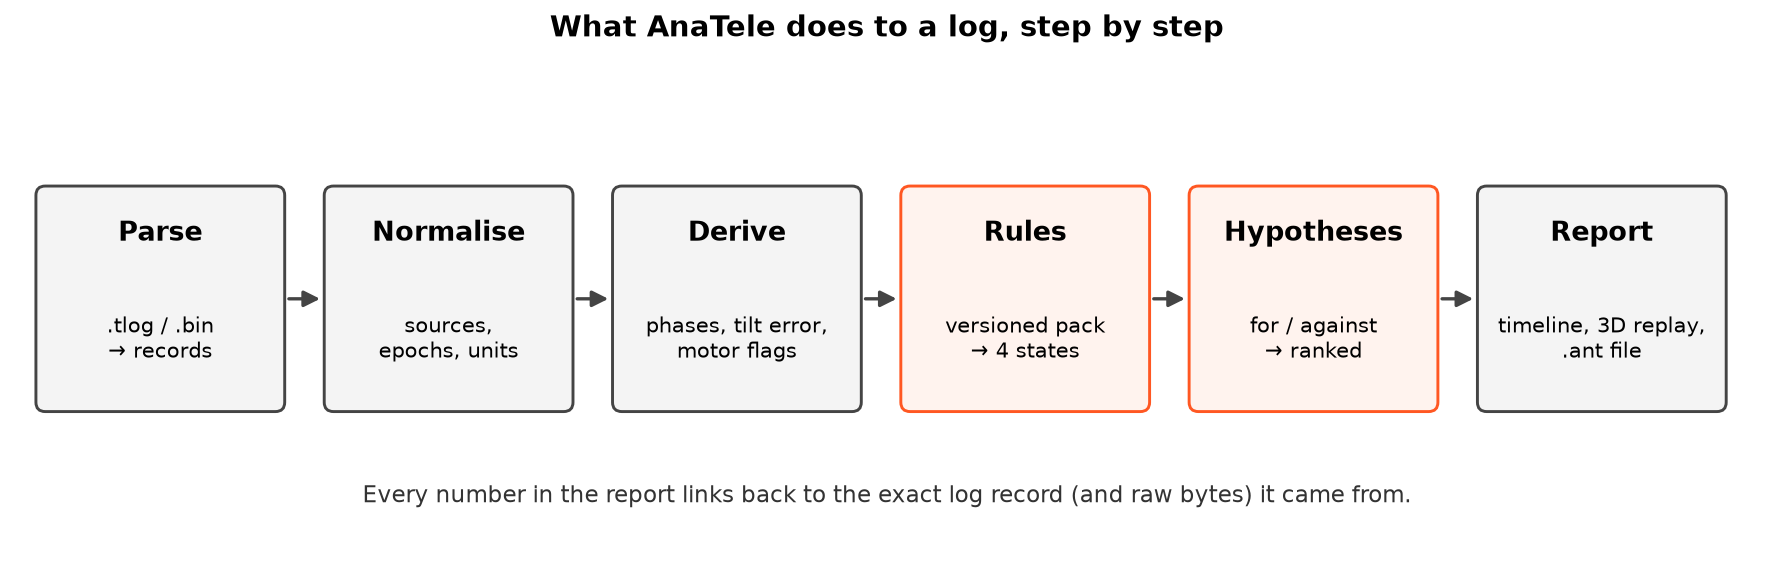
\includegraphics[width=0.75\linewidth]{images/guide/08_pipeline.png}\par\vspace{1.5cm}
{\Huge\bfseries AnaTele Illustrated Guide\par}\vspace{0.4cm}
{\Large Learn drone flight-log investigation from scratch\par}\vspace{1.2cm}
{\large Avinash Chandra Gupta\par}\vspace{0.3cm}
{\normalsize \url{https://avinashistoocool.github.io/AnaTele/learn/}\par}
\vfill
{\small Every chart is drawn from real simulator flights analysed by AnaTele itself.\\
Generated from the web guide by \texttt{docs/figures/build\_guide\_tex.py}.\par}
\end{titlepage}
\tableofcontents

\chapter{Introduction}

This is an illustrated course. It assumes \textbf{no} background: you don't need to have flown a drone, opened a log
or seen the maths before. By the end you'll be able to read an AnaTele report and explain every number in it.

Every chart is drawn from \textbf{real data}: flights from AnaTele's built-in simulator, analysed by the
same code you run. The script that draws them is
\href{https://github.com/Avinashistoocool/AnaTele/tree/main/docs/figures}{\texttt{docs/figures/make\_\allowbreak{}guide\_\allowbreak{}figures.py}}.
Some pages also have small interactive widgets that run in your browser.


\section{How to use this course}

\begin{itemize}
\item \textbf{In a hurry?} Read chapters 1, 4, 5 and 9. That's enough to read a crash report.
\item \textbf{Investigating a real crash?} Do chapters 4--9 next to the \href{https://avinashistoocool.github.io/AnaTele/DIAGNOSTICS/}{Diagnostics reference}.
\item \textbf{Writing your own rules?} Read chapters 8 and 9, then \href{https://avinashistoocool.github.io/AnaTele/DIAGNOSTICS/\#writing-a-rule}{Writing a rule}.
\end{itemize}

\begin{guidebox}{The one idea to keep in mind}{blue!50!black}
AnaTele reports \textbf{observations} and \textbf{hypotheses}. It never gives a crash verdict or a probability of cause.
If data is missing, the answer is \emph{unknown}, never \emph{fine}.
\end{guidebox}
\chapter{Drones 101}
\label{ch:01-drones-101}

\section{The parts}

A quadcopter is four motors with propellers on arms, a battery, and a small computer called the **flight
controller\textbf{. AnaTele works with flight controllers running }ArduPilot**, the open-source autopilot used in
everything from hobby quads to survey drones.

\begin{figure}[H]\centering
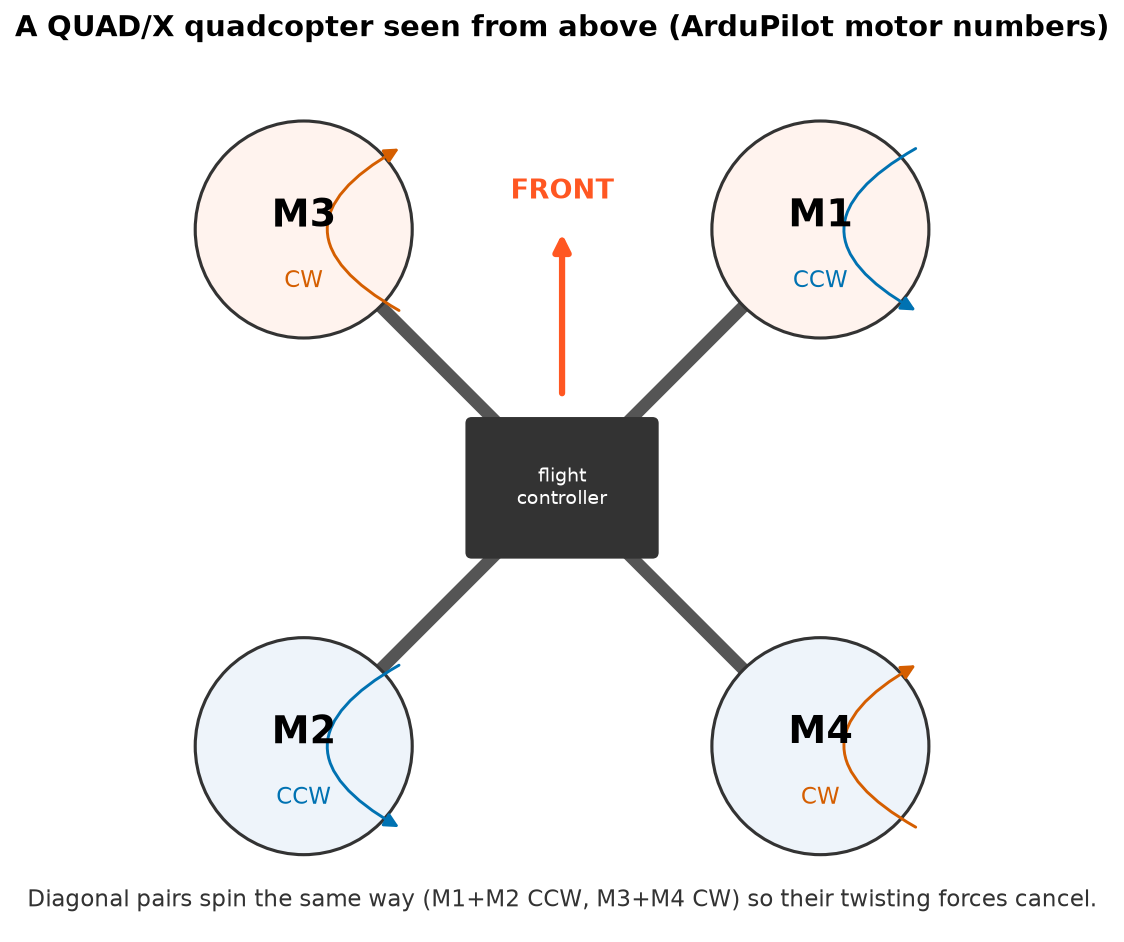
\includegraphics[width=\linewidth,height=0.42\textheight,keepaspectratio]{images/guide/01_quad_layout.png}
\caption{QUAD/X layout}
\end{figure}

ArduPilot numbers the motors of an ``X'' quad the way the figure shows. Motor 1 is front-right, not front-left,
which surprises most people. Diagonal pairs spin the same way: M1 and M2 counter-clockwise (CCW), M3 and M4
clockwise (CW). Each spinning propeller twists the frame the opposite way. With two of each direction, the twists
cancel and the drone doesn't spin.

\begin{guidebox}{Why this matters in an investigation}{green!40!black}
If a motor is wired to the wrong output, or a propeller is on the wrong motor, the drone usually flips
on takeoff. AnaTele reads \texttt{SERVOn\_\allowbreak{}FUNCTION}, \texttt{FRAME\_\allowbreak{}CLASS} and \texttt{FRAME\_\allowbreak{}TYPE} from the log so that every motor
number it shows matches this picture.

\end{guidebox}
\section{Three angles: roll, pitch, yaw}

The \textbf{attitude} of a drone is which way it's facing and how it's tilted. Three angles describe it:

\begin{figure}[H]\centering
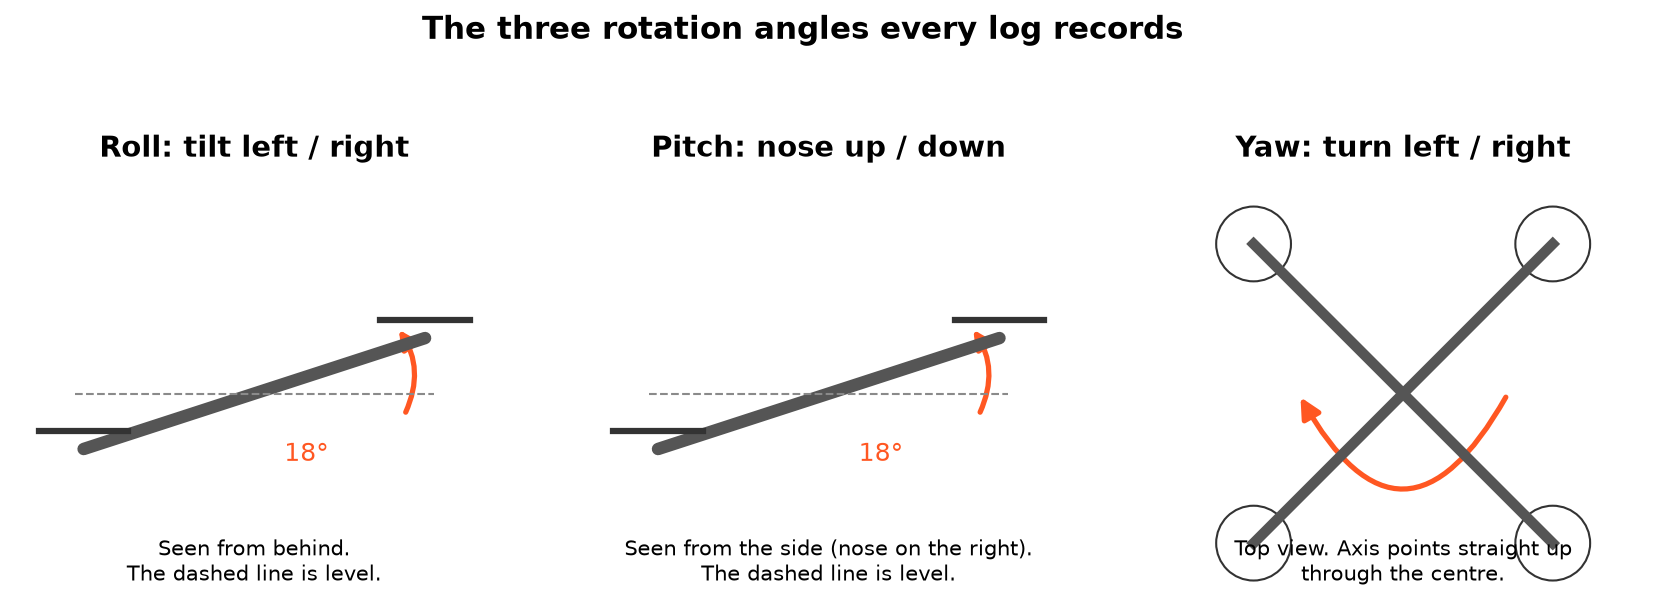
\includegraphics[width=\linewidth,height=0.42\textheight,keepaspectratio]{images/guide/02_roll_pitch_yaw.png}
\caption{Roll, pitch and yaw}
\end{figure}

\begin{itemize}
\item \textbf{Roll}: tilting left or right, like a plane banking.
\item \textbf{Pitch}: nose up or nose down.
\item \textbf{Yaw}: turning left or right while staying level. This is the drone's \emph{heading}.
\end{itemize}

A quadcopter has no rudder or wings, so it moves by \textbf{tilting}. To fly forward it pitches its nose down. Part of the
thrust then points backwards and pushes it forward. That is why ``is the tilt correct?'' is the most important
question in chapter 5.

\section{Thrust, weight and hover}

To hover, the motors must push up exactly as hard as gravity pulls down.

\begin{figure}[H]\centering
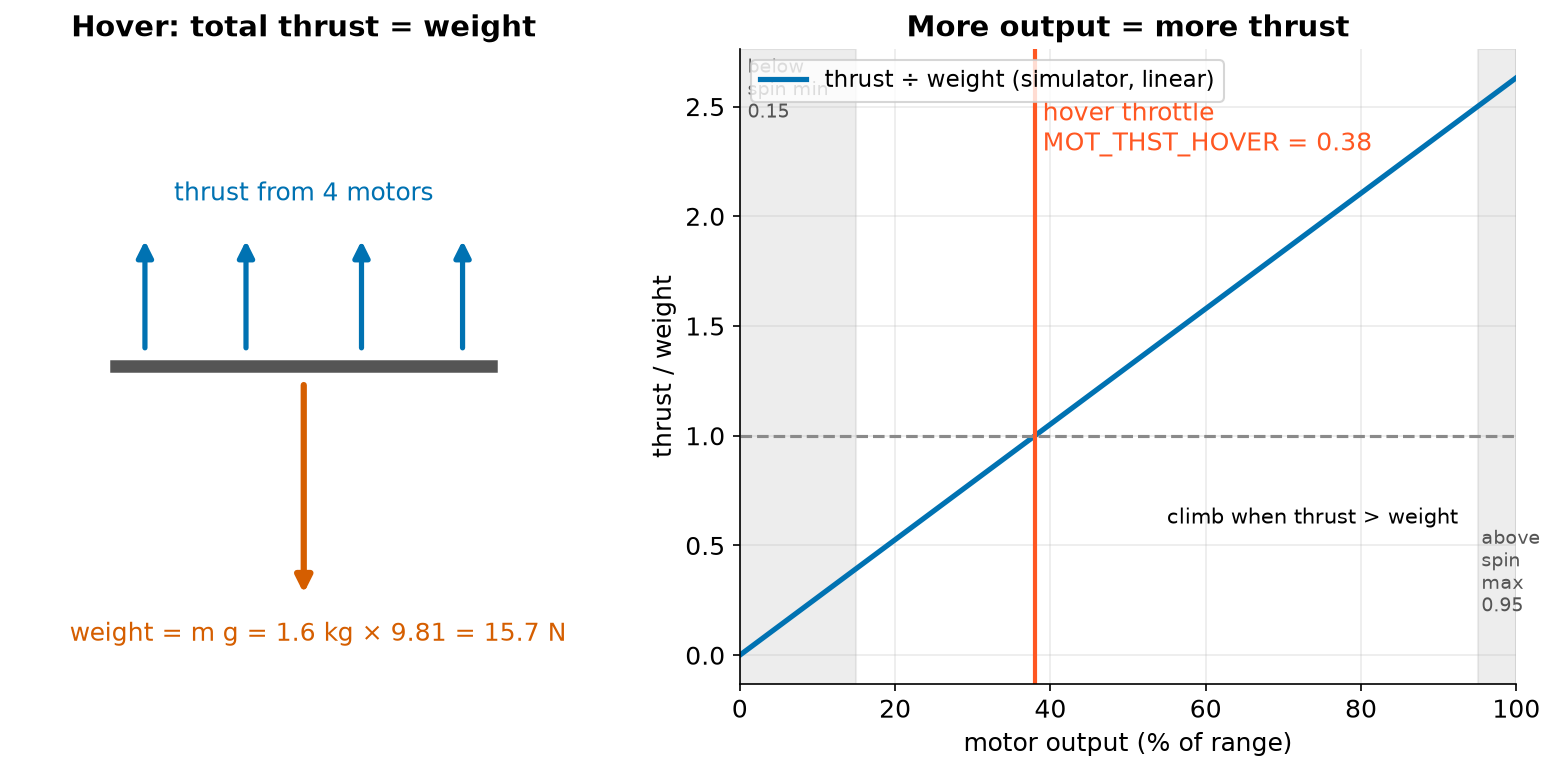
\includegraphics[width=\linewidth,height=0.42\textheight,keepaspectratio]{images/guide/03_thrust_balance.png}
\caption{Thrust balance}
\end{figure}

The simulator's drone weighs 1.6 kg, so its weight is

\[
 W = m g = 1.6\,\text{kg} \times 9.81\,\text{m/s}^2 \approx 15.7\,\text{N}. 
\]

ArduPilot records the motor output needed to hover as \texttt{MOT\_\allowbreak{}THST\_\allowbreak{}HOVER}. In the simulated flights it is \textbf{0.38}:
38 \% of the usable range. More output gives more thrust and the drone climbs. Less output and it descends.

Motors also have limits. Below \texttt{MOT\_\allowbreak{}SPIN\_\allowbreak{}MIN} (0.15 here) they can stall. Above \texttt{MOT\_\allowbreak{}SPIN\_\allowbreak{}MAX} (0.95) there's
no headroom left. A motor that sits at one of these limits is \textbf{saturated}. Chapter 6 shows why that's an
important clue.

\begin{guidebox}{Check your understanding}{violet!70!black}
The drone is hovering and you want it to roll right. Which motors must push harder?
\begin{guidebox}{Answer}{green!40!black}
The \textbf{left} ones (M2 back-left and M3 front-left). Pushing up harder on the left tips the drone to the right.
\end{guidebox}
\end{guidebox}
\chapter{Logs and MAVLink}
\label{ch:02-logs-and-mavlink}

\section{What is a flight log?}

During a flight, the flight controller reads its sensors hundreds of times a second. It estimates where it is,
decides what to do and drives the motors. It also writes a record of all of this, and that record is the
\textbf{flight log}.

\begin{figure}[H]\centering
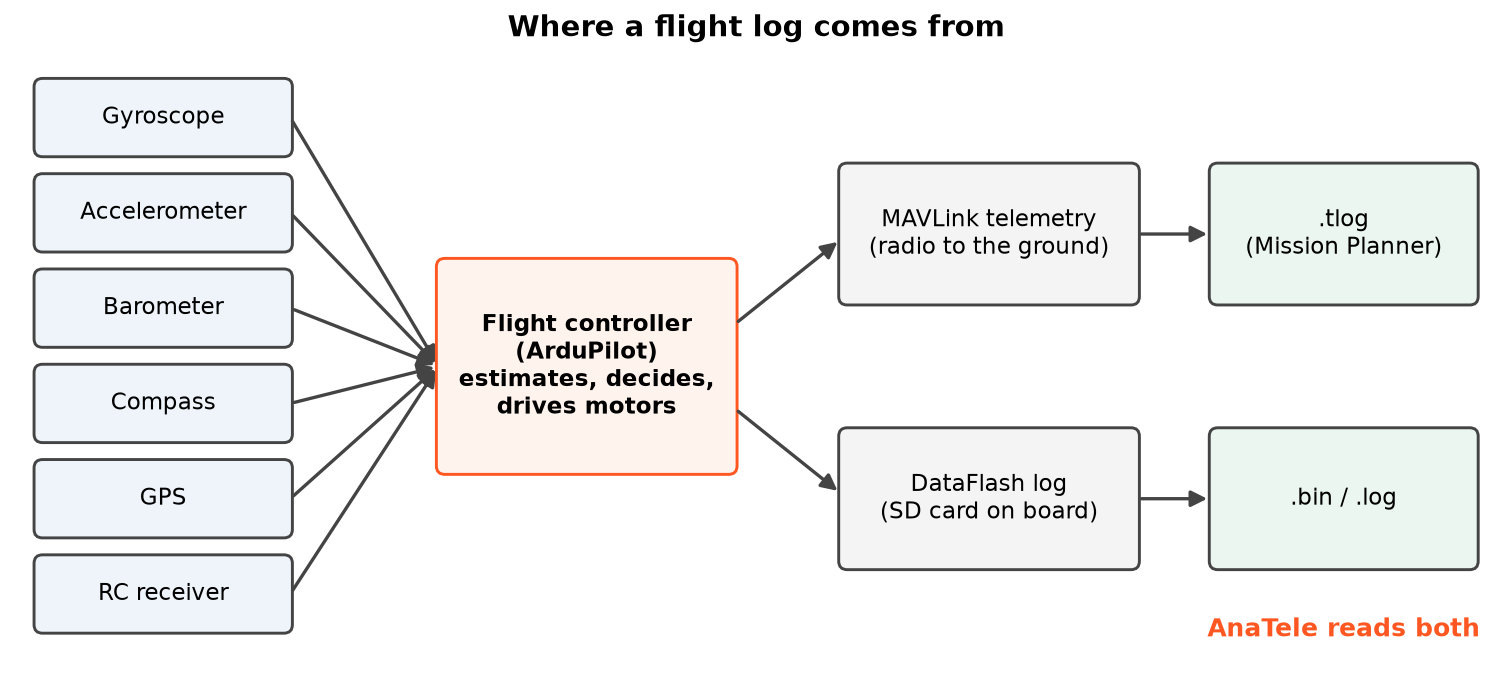
\includegraphics[width=\linewidth,height=0.42\textheight,keepaspectratio]{images/guide/04_what_is_a_log.png}
\caption{Where a log comes from}
\end{figure}

There are two kinds, and AnaTele reads both:

\begin{center}\small
\begin{tabularx}{\linewidth}{XXX}
\toprule
Log & Where it is made & What it contains \\
\midrule
\textbf{Telemetry log} \texttt{.tlog} & On the ground station (e.g. Mission Planner), from the radio link & \textbf{MAVLink} messages, each stamped with the time the ground received it \\
\textbf{DataFlash log} \texttt{.bin} / \texttt{.log} & On the drone's SD card & ArduPilot's own on-board records; usually higher rate and more detail \\
\bottomrule
\end{tabularx}
\end{center}

\textbf{MAVLink} is the language drones and ground stations use to talk. Each MAVLink message has a type (for example
\texttt{ATTITUDE} or \texttt{GPS\_\allowbreak{}RAW\_\allowbreak{}INT}) and named fields (\texttt{roll}, \texttt{pitch}, \texttt{lat}, \texttt{lon}\ldots{}).

\section{A log is a stream of typed messages}

Here is the start-to-finish stream of a simulated flight in which one motor fails. Each tick is one message.

\begin{figure}[H]\centering
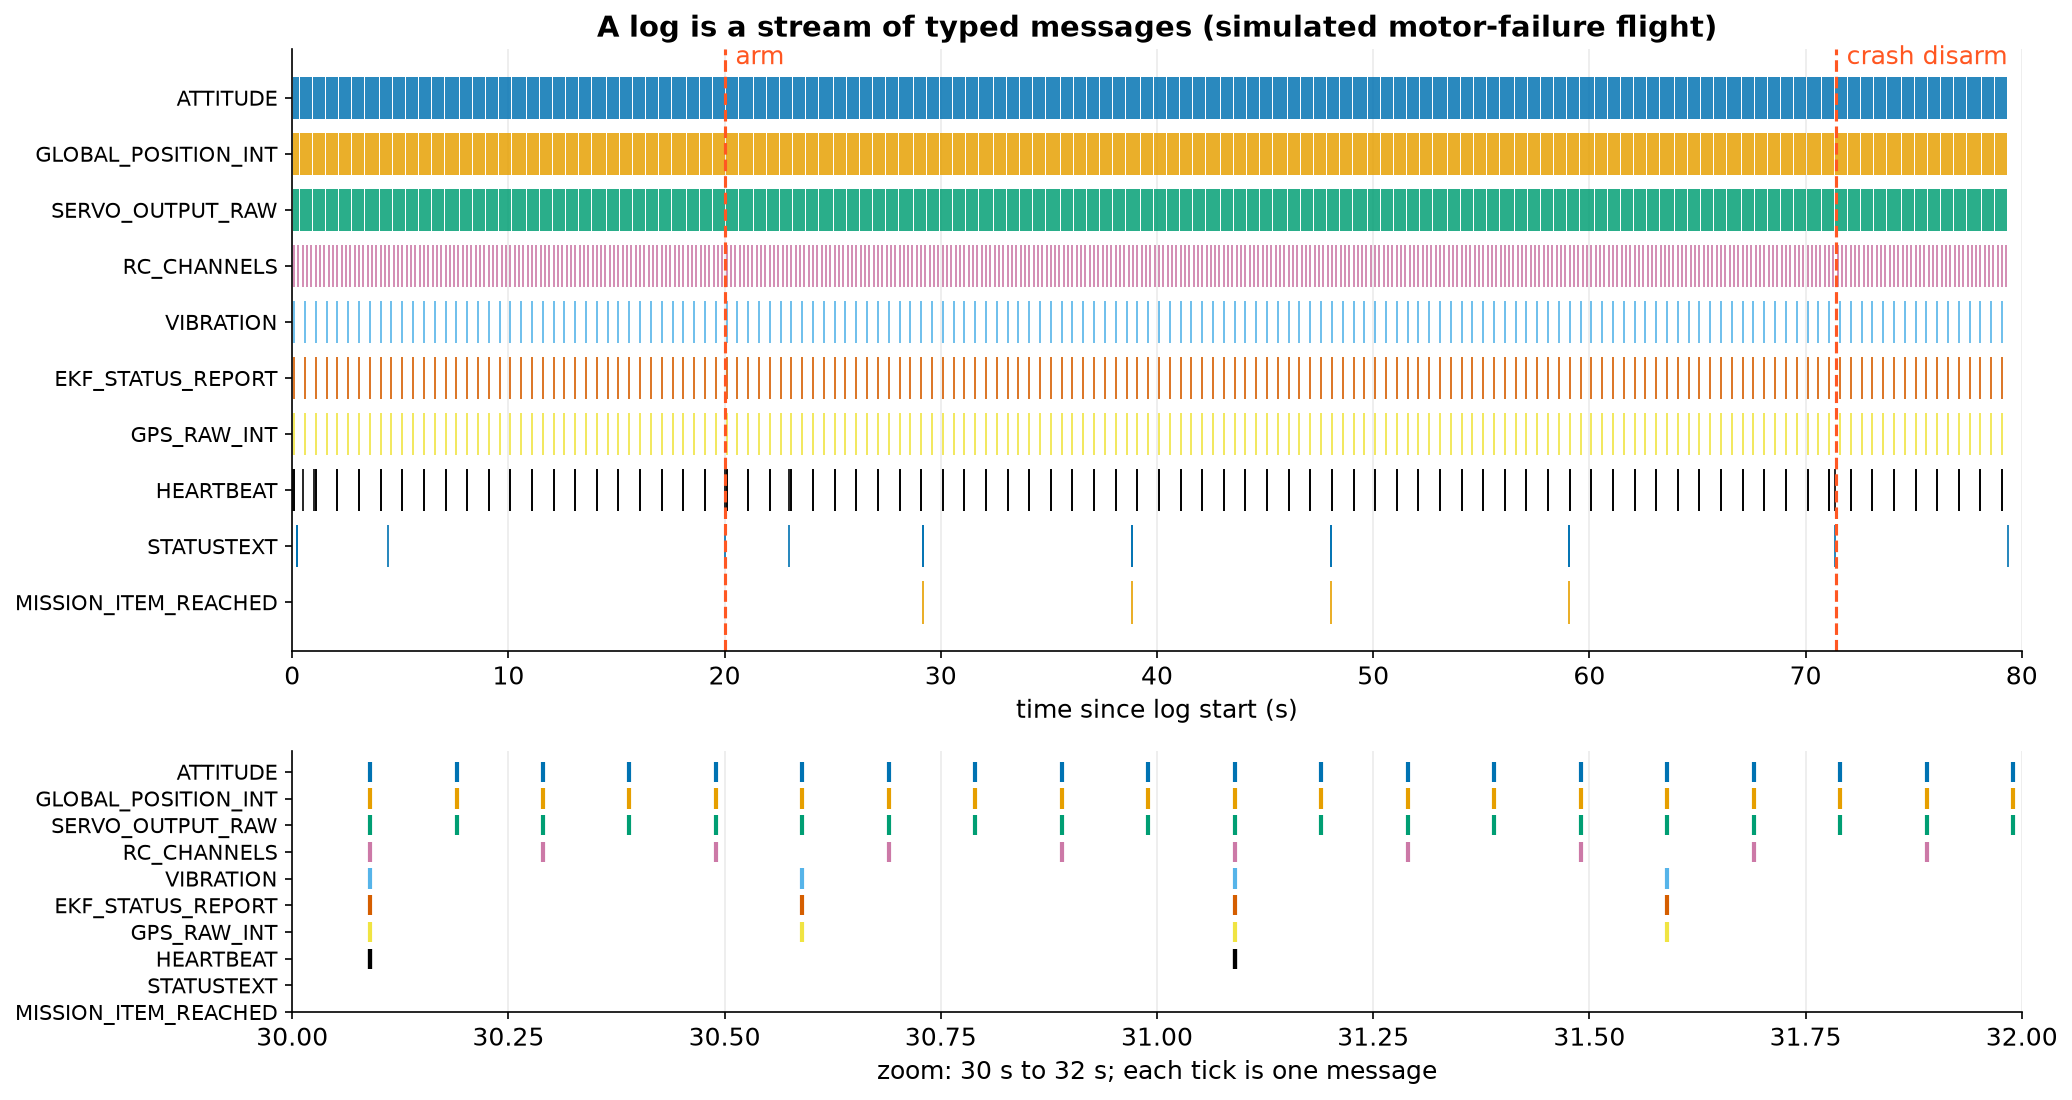
\includegraphics[width=\linewidth,height=0.42\textheight,keepaspectratio]{images/guide/05_message_stream.png}
\caption{Message stream}
\end{figure}

Things to notice:

\begin{itemize}
\item \texttt{ATTITUDE}, \texttt{GLOBAL\_\allowbreak{}POSITION\_\allowbreak{}INT} and \texttt{SERVO\_\allowbreak{}OUTPUT\_\allowbreak{}RAW} are dense bands: they arrive many times a second.
\item \texttt{STATUSTEXT} (human-readable text such as \emph{``Crash: Disarming''}) shows up only a handful of times, but these
messages are often the most important ones.
\item \texttt{MISSION\_\allowbreak{}ITEM\_\allowbreak{}REACHED} marks each waypoint the autopilot reports reaching.
\end{itemize}

\section{Different messages, different rates}

\begin{figure}[H]\centering
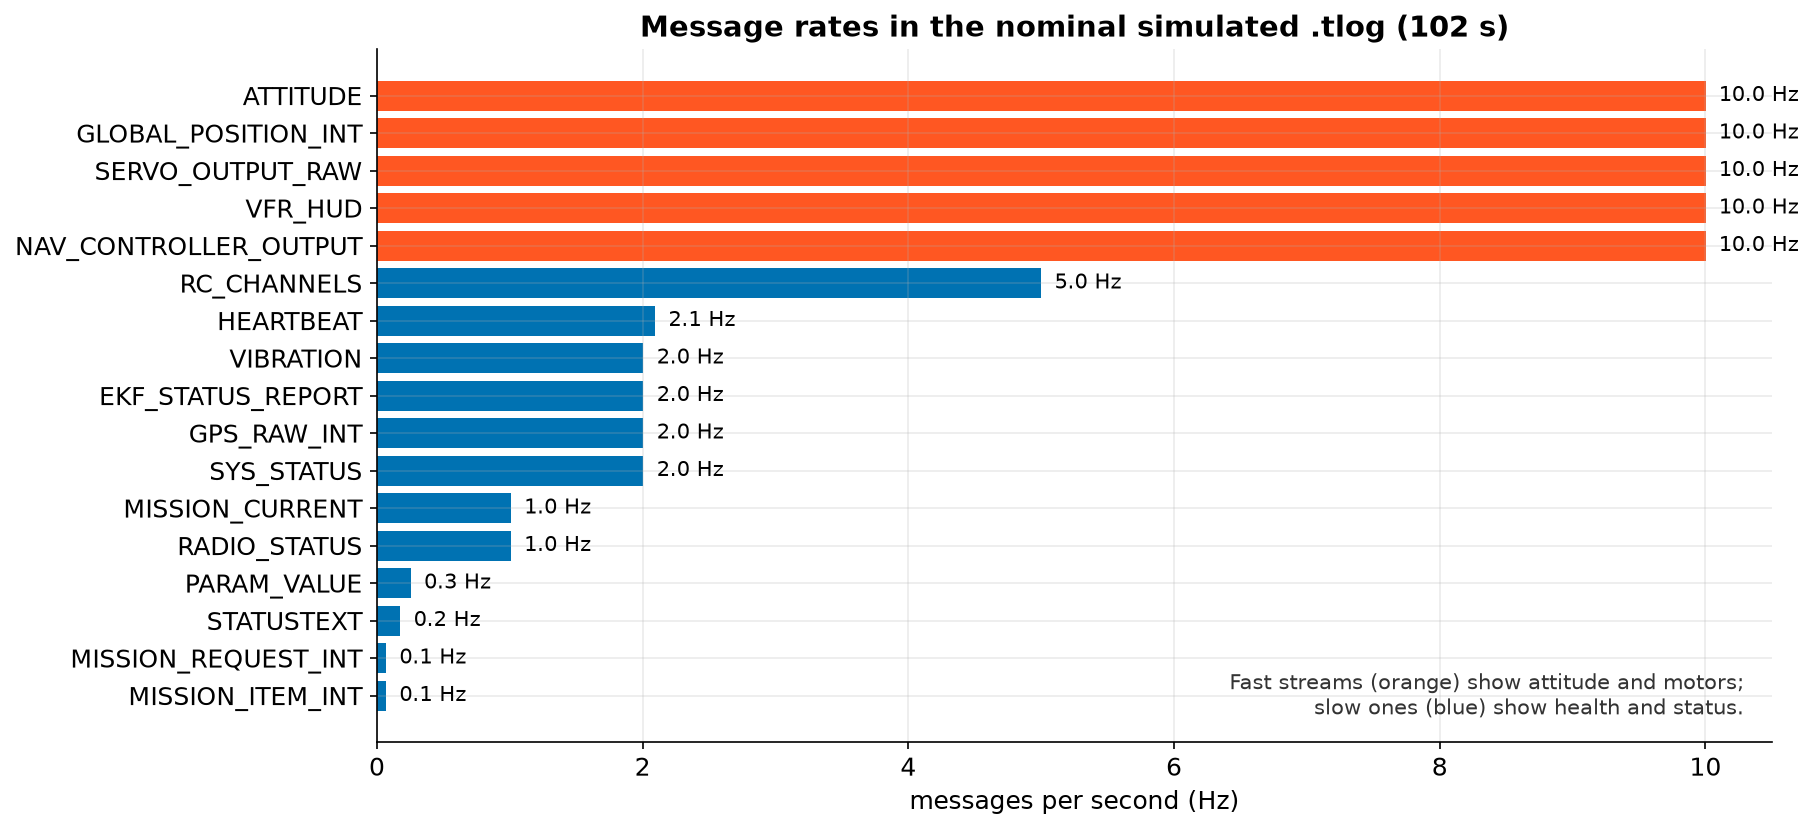
\includegraphics[width=\linewidth,height=0.42\textheight,keepaspectratio]{images/guide/06_sample_rates.png}
\caption{Sample rates}
\end{figure}

In this 102-second simulated \texttt{.tlog}, attitude, position, motor outputs and the controller's targets arrive at
\textbf{10 Hz} (10 times a second). RC input arrives at 5 Hz, and vibration, EKF status, GPS and battery at \textbf{2 Hz}.

\begin{guidebox}{Rate limits what you can conclude}{orange!80!black}
A rule that needs ``above 30 for at least 0.5 s'' can't be checked properly with data every 0.5 s. AnaTele
knows this. When the data is too sparse, it marks the rule \textbf{unassessable} instead of pretending it's healthy
(chapter 8).

\end{guidebox}
\section{What AnaTele keeps}

When AnaTele opens a log it keeps \textbf{every decoded record}, with its byte offset in the file. The simulated
motor-failure log has 5,387 records. Every chart, threshold and hypothesis in the report can therefore be traced
back to the exact bytes it came from. This is the \emph{evidence viewer} in the desktop app.
\chapter{Time and sources}
\label{ch:03-time-and-sources}

\section{Two clocks}

Every record in a log has a time, but not always from the same clock.

\begin{figure}[H]\centering
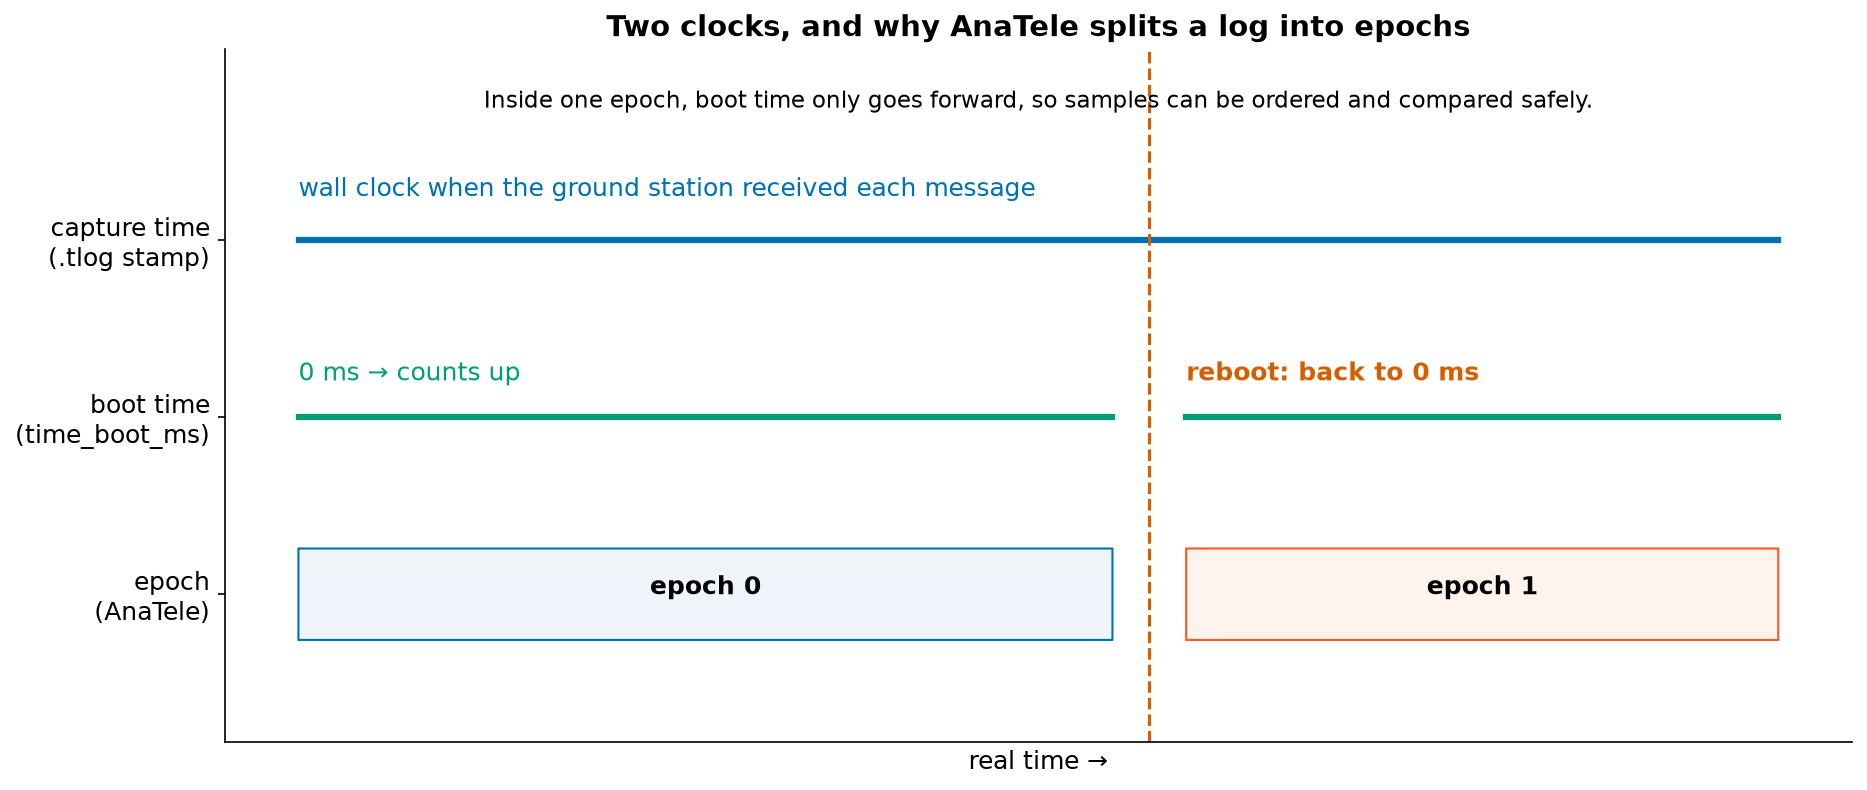
\includegraphics[width=\linewidth,height=0.42\textheight,keepaspectratio]{images/guide/07_time_bases.png}
\caption{Time bases}
\end{figure}

\begin{itemize}
\item \textbf{Capture time}: when the ground station received the message (the 8-byte stamp in front of each \texttt{.tlog}
record). It's wall-clock time, so it can jump if the PC's clock is adjusted, and it includes radio delay.
\item \textbf{Boot time} (\texttt{time\_\allowbreak{}boot\_\allowbreak{}ms}, \texttt{time\_\allowbreak{}usec}): how long the flight controller has been powered on. It's
precise, but it \textbf{restarts from zero} when the board reboots.
\end{itemize}

\section{Epochs}

If the board reboots mid-log, ``10 s after boot'' happens twice. Put both runs on one timeline and you'd mix two
different flights. AnaTele avoids this by splitting the log into \textbf{epochs}. A new epoch starts whenever a clock
clearly goes backwards. Inside one epoch, time only moves forward, so samples can be ordered, paired and compared
safely.

The exact tests (per source) are:

\begin{center}\small
\begin{tabularx}{\linewidth}{XXX}
\toprule
Clock & New epoch when\ldots{} & Why the margin \\
\midrule
\texttt{.tlog} boot time \texttt{time\_\allowbreak{}boot\_\allowbreak{}ms} & it drops by more than \textbf{10 s} & Small regressions are just reordered / delayed packets \\
DataFlash boot time & it drops by more than \textbf{1 s} & On-board records are written in order \\
\texttt{.tlog} capture time & it drops by more than \textbf{2 s} & PC clock adjustments separate the whole capture \\
\bottomrule
\end{tabularx}
\end{center}

A boot-time drop from near $2^{32}$ ms back to near zero is recognised as a counter \textbf{wrap} (after \textasciitilde{}49.7 days),
not a reboot. Every epoch split is listed as a diagnostic, so you can see why it happened.

\section{Sources}

A capture can hold messages from more than one system: the drone, a gimbal, the ground station, a companion
computer. MAVLink identifies each sender by a \emph{system id} and \emph{component id}. AnaTele calls each pair a
\textbf{source} (for example \texttt{1:1} is the autopilot) and never mixes signals from different sources.

\section{Pairing samples}

Many checks compare two signals, for example desired and actual roll. They don't arrive at exactly the same
instant, so AnaTele pairs each sample with the \textbf{nearest} sample of the other signal, within a tolerance. For
attitude that tolerance is \textbf{0.25 s}. If no partner is close enough, the pair is skipped rather than guessed.

\begin{guidebox}{Design principle}{blue!50!black}
Nothing is interpolated or invented. A derived value always comes from real samples, close enough in time to
be compared, and it keeps a link to the record it came from.
\end{guidebox}
\chapter{Flight phases}
\label{ch:04-flight-phases}

A crash investigation is about \textbf{timing}: what was normal, when did it stop being normal, what came first.
So the first thing AnaTele does with each armed period (an \emph{episode}) is split it into phases.

\begin{figure}[H]\centering
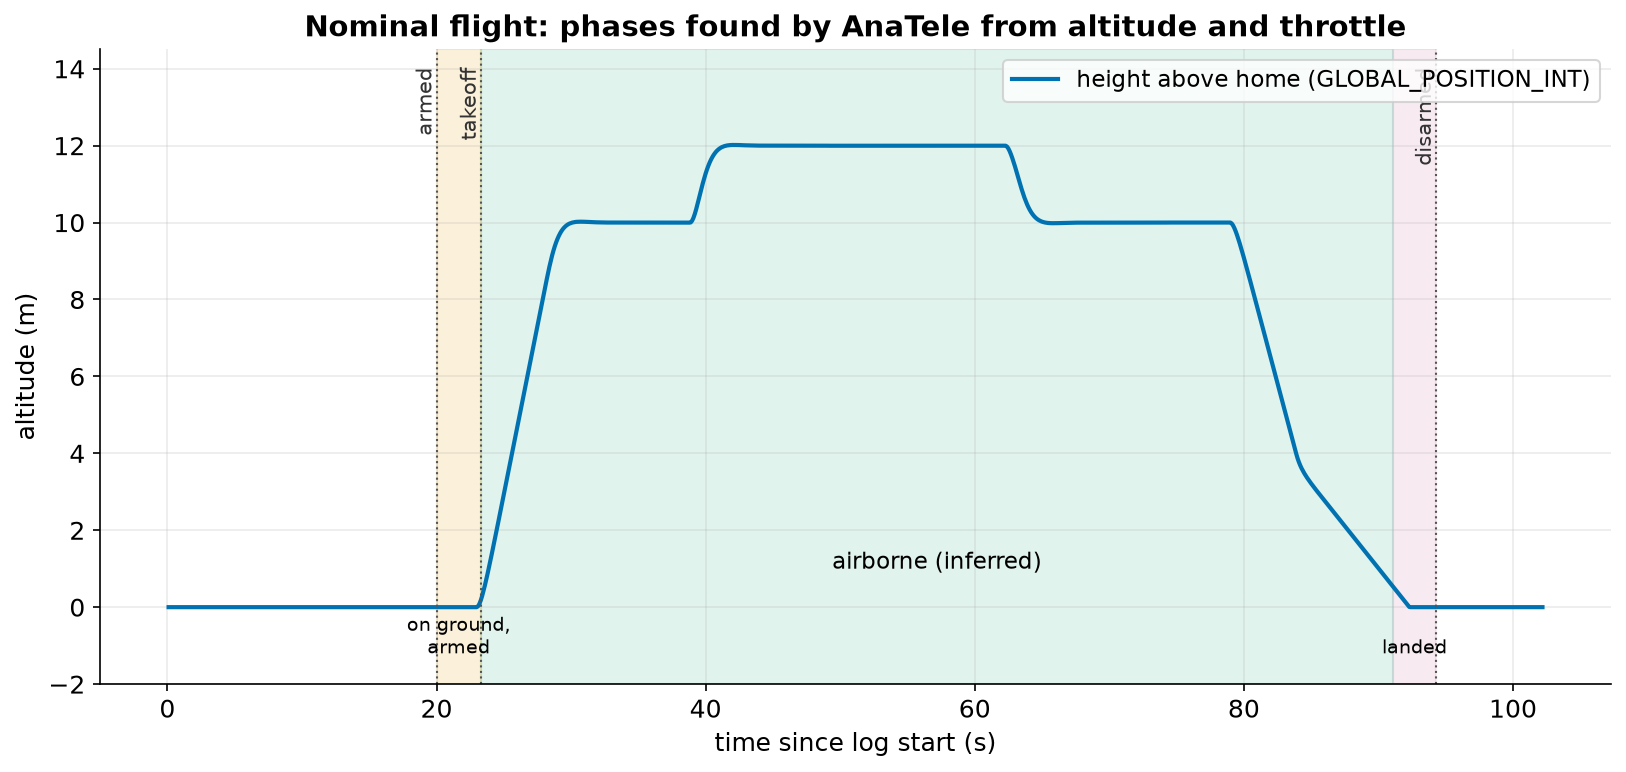
\includegraphics[width=\linewidth,height=0.42\textheight,keepaspectratio]{images/guide/09_altitude_phases.png}
\caption{Altitude and phases}
\end{figure}

In the nominal simulated flight, the drone arms at 20.0 s and AnaTele finds takeoff at \textbf{23.29 s}. It's
airborne until 91.09 s and disarms at 94.27 s.

\section{Step 1: the armed baseline}

Altitude estimates drift, so ``altitude = 0'' doesn't reliably mean ``on the ground''. AnaTele takes the \textbf{median}
home-relative altitude during the first \textbf{2 s} after arming as the ground level (the \emph{baseline}). The median is
used instead of the mean so a single bad sample can't move it.

\section{Step 2: confirm, then backtrack}

\begin{figure}[H]\centering
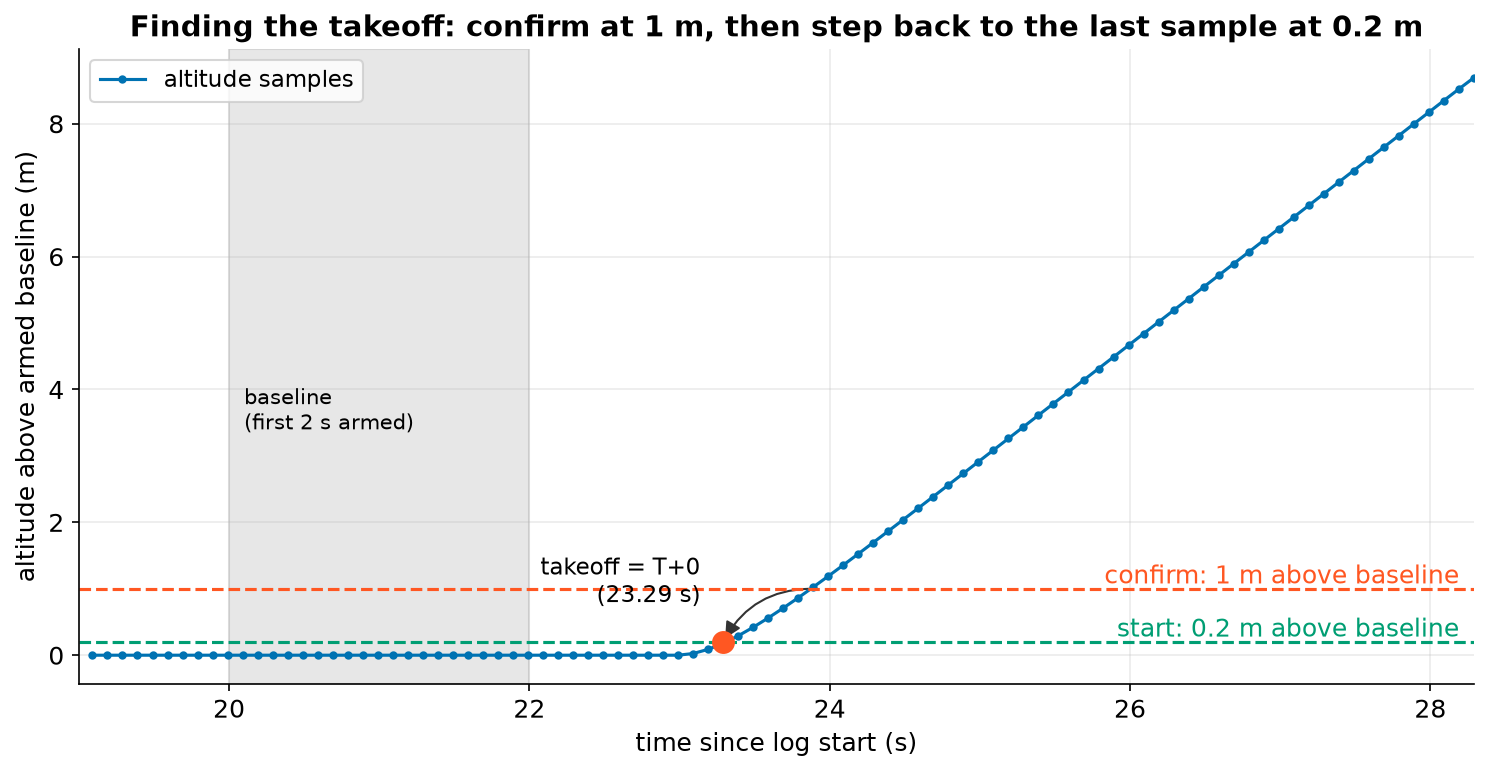
\includegraphics[width=\linewidth,height=0.42\textheight,keepaspectratio]{images/guide/10_takeoff_detection.png}
\caption{Takeoff detection}
\end{figure}

\begin{enumerate}
\item Find the first sample at least \textbf{1.0 m} above the baseline. That is clearly flying, not noise.
\item Check that there was real \textbf{demand} in the 5 s before it: throttle at least \textbf{10 \%}, or (if throttle isn't
logged) a motor output of at least 25 \% of its range. If the altitude rose with no demand, it's treated as
estimate drift and the drone is \emph{not} considered airborne.
\item Walk \textbf{backwards} to the last sample still within \textbf{0.2 m} of the baseline. That's the takeoff time, \textbf{T+0}.
\end{enumerate}

If the autopilot itself reports ``Taking off'' or ``In air'' (a landed-state message), AnaTele uses that instead and
labels the phase \emph{reported} rather than \emph{inferred}.

\section{Step 3: the pre-event window}

Rules mostly look at the time \textbf{before} anything went wrong. Once the drone has hit the ground, all the
sensors go wild, and that's a consequence, not a cause.

\begin{figure}[H]\centering
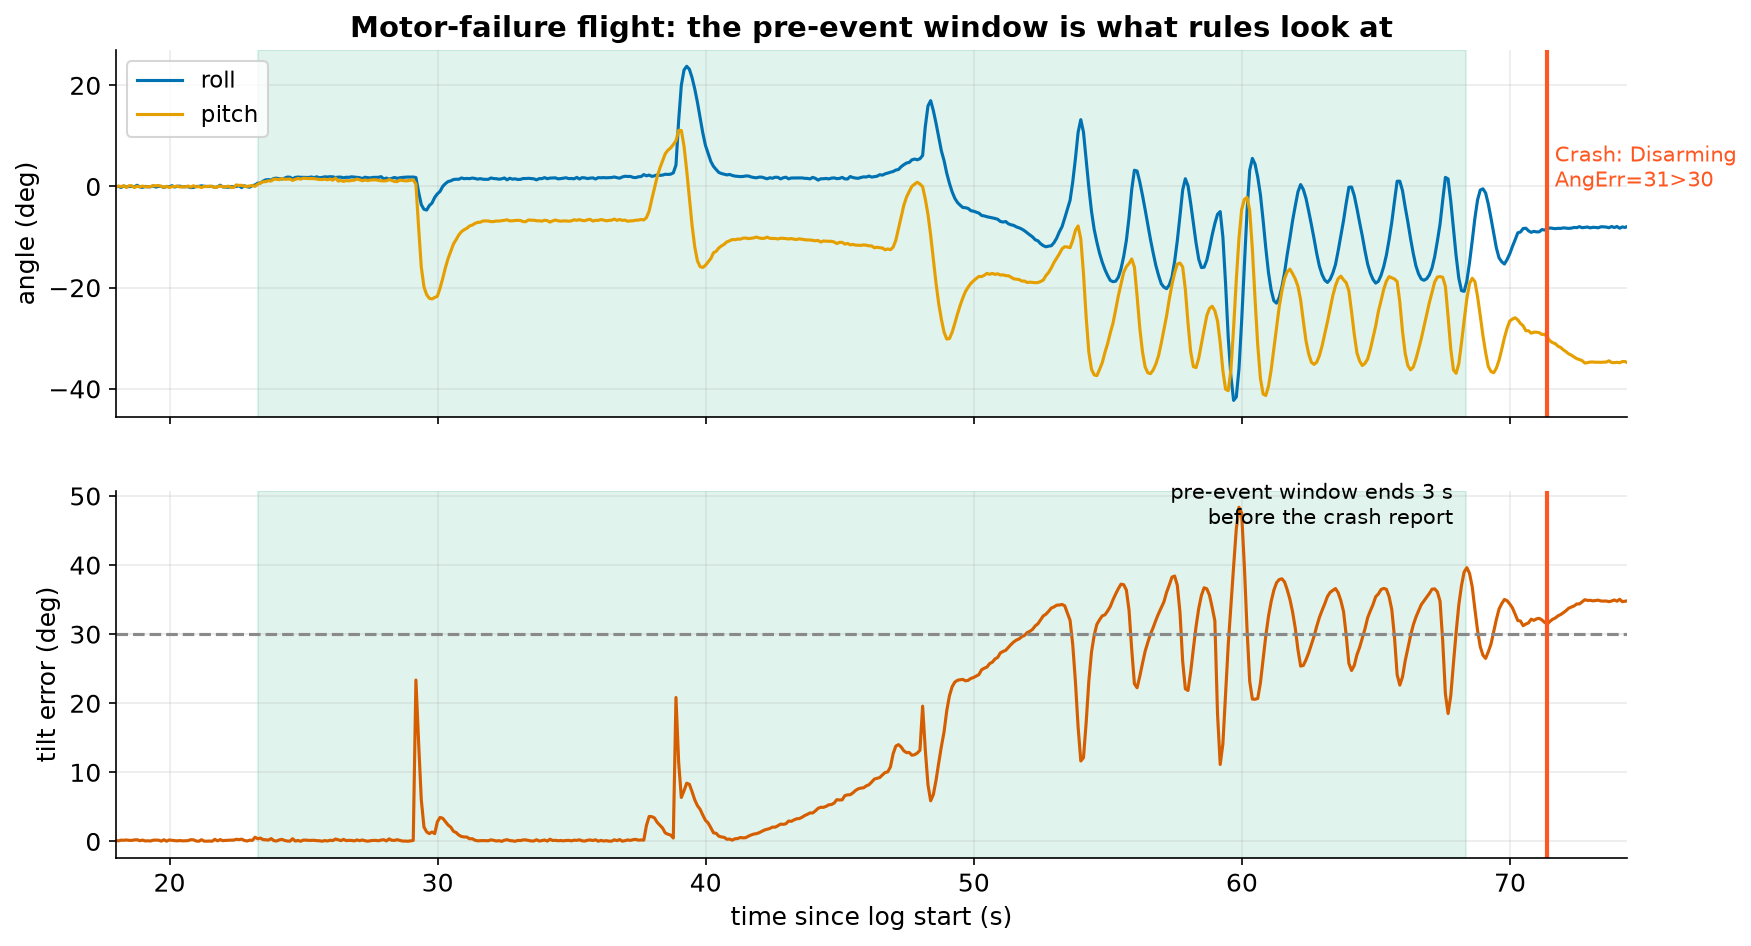
\includegraphics[width=\linewidth,height=0.42\textheight,keepaspectratio]{images/guide/11_upset_detection.png}
\caption{Upset detection}
\end{figure}

The window ends at the earliest of:

\begin{itemize}
\item the first moment roll or pitch exceeds \textbf{60\textdegree{}} (an attitude excursion, i.e. loss of control);
\item \textbf{3 s} before an autopilot crash report (the \emph{event guard});
\item the last sample at least 0.5 m above the baseline.
\end{itemize}

In the motor-failure flight, ArduPilot reported \emph{``Crash: Disarming: AngErr=31>30''} at 71.37 s. The roll and pitch
never passed 60\textdegree{}, so the pre-event window runs from takeoff (23.29 s) to \textbf{68.37 s}, exactly 3 s before the
report.

\begin{guidebox}{Phase labels in the report}{blue!50!black}
\begin{itemize}
\item \texttt{airborne\_\allowbreak{}reported}: from the autopilot's own landed-state messages.
\item \texttt{airborne\_\allowbreak{}inferred}: from altitude rise plus demand, as above.
\item \texttt{no\_\allowbreak{}airborne\_\allowbreak{}evidence}: armed, but never clearly flew.
\item \texttt{unassessable}: no altitude data, so we can't tell.
\end{itemize}
\end{guidebox}
\chapter{Attitude and tilt error}
\label{ch:05-attitude-and-tilt-error}

\section{Desired versus actual}

The autopilot constantly decides what attitude it \textbf{wants} (desired roll and pitch). It then tries to achieve it
with the motors. A healthy drone follows closely:

\begin{figure}[H]\centering
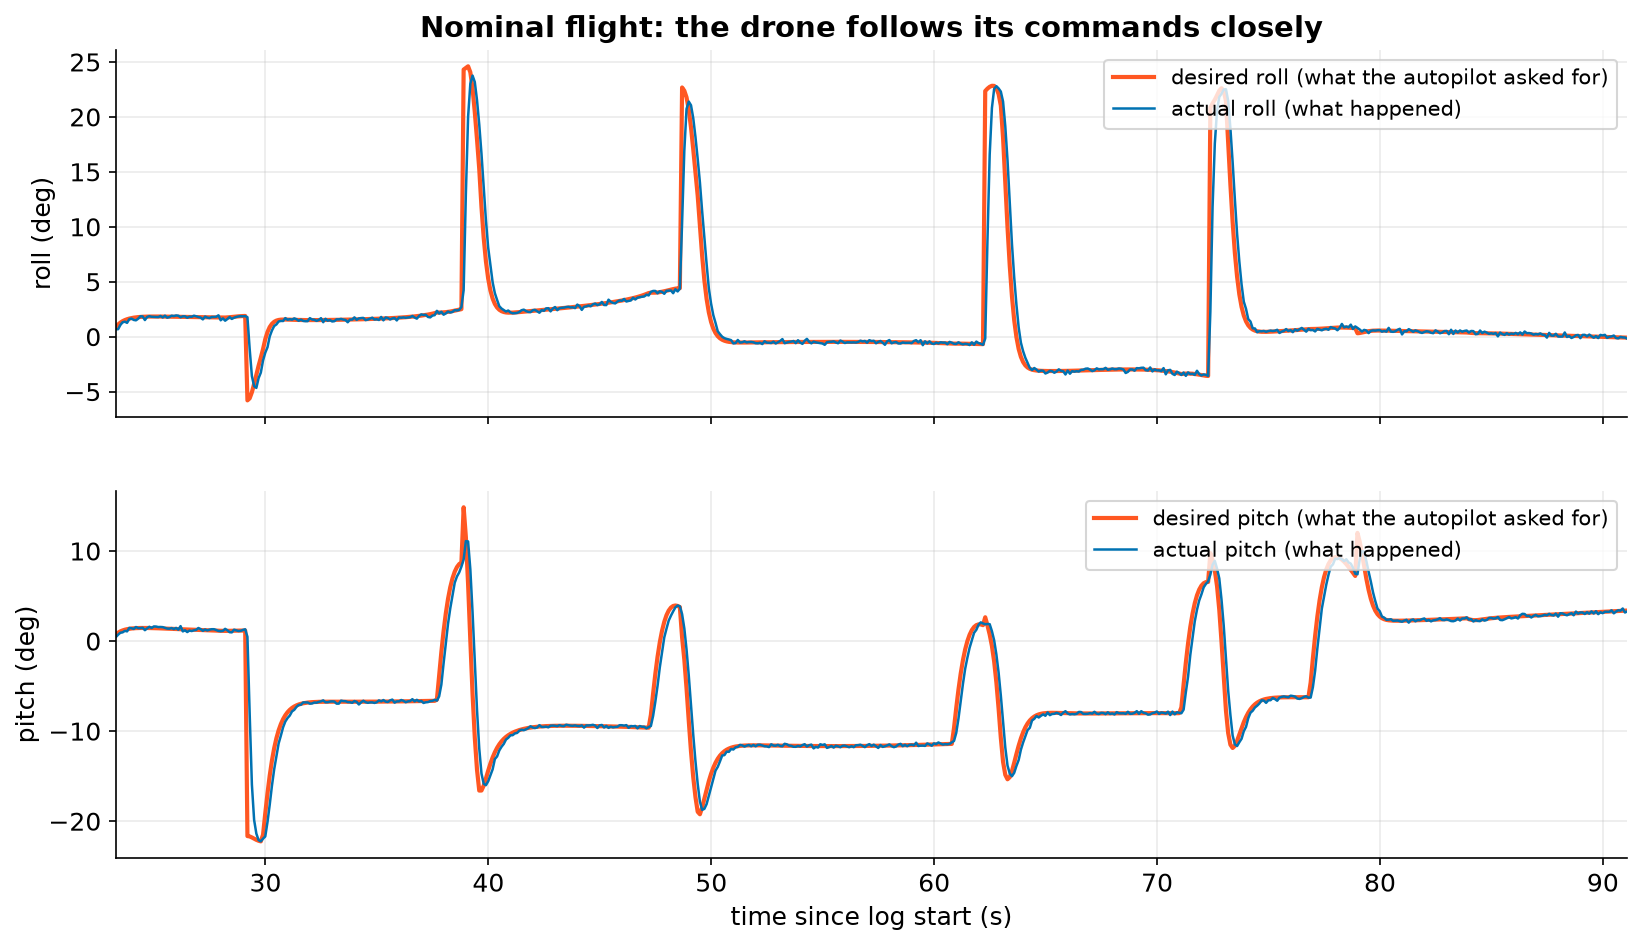
\includegraphics[width=\linewidth,height=0.42\textheight,keepaspectratio]{images/guide/12_desired_vs_actual.png}
\caption{Desired vs actual}
\end{figure}

When a motor is failing, a propeller is damaged or the frame is wrongly configured, the drone can no longer follow.
The gap between ``wanted'' and ``got'' grows. This is one of the strongest clues in an investigation.

\section{One number: the tilt error}

Roll and pitch errors could be checked separately, but what really matters is \textbf{which way the thrust points}. So
AnaTele turns each (roll, pitch) pair into a unit vector along the drone's thrust axis:

\[
 \hat{t}(\phi, \theta) = \big( \sin\theta \cos\phi,\; -\sin\phi,\; \cos\theta \cos\phi \big) 
\]

where $\phi$ is roll and $\theta$ is pitch. The \textbf{tilt error} is the angle between the desired and actual vectors:

\[
 e = \arccos\!\big( \hat{t}_\text{desired} \cdot \hat{t}_\text{actual} \big). 
\]

\begin{figure}[H]\centering
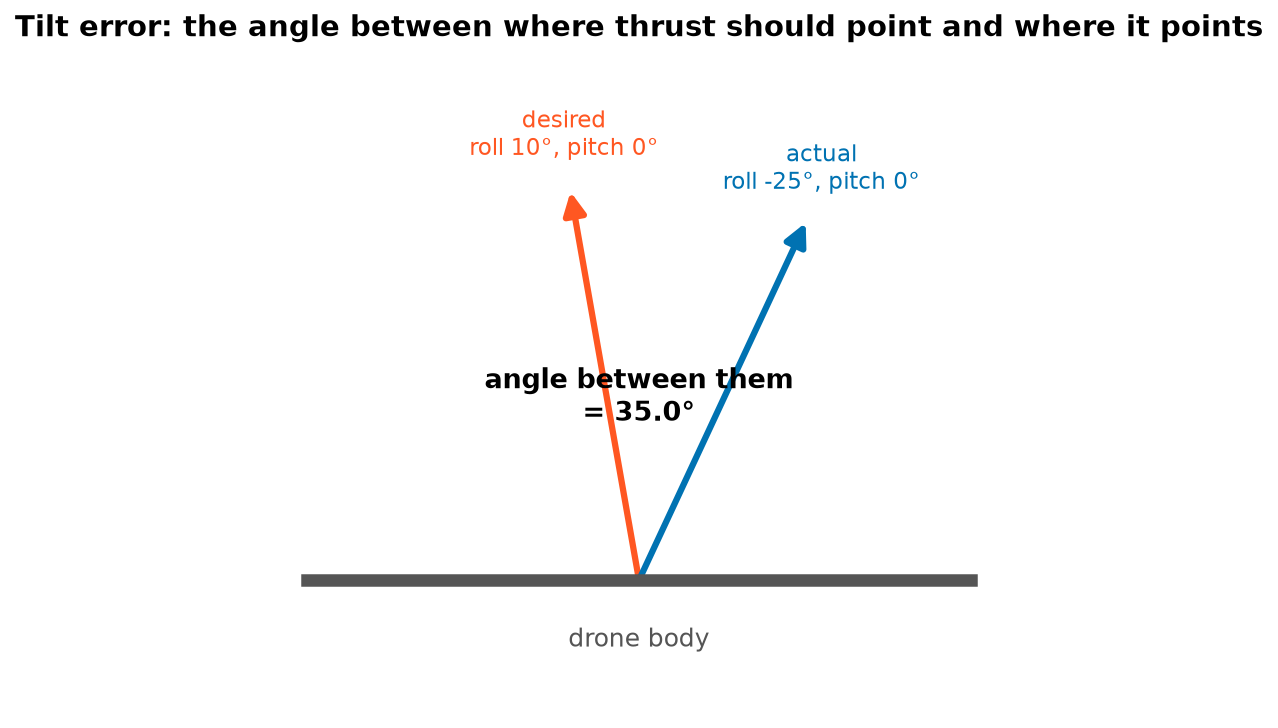
\includegraphics[width=\linewidth,height=0.42\textheight,keepaspectratio]{images/guide/13_tilt_error_geometry.png}
\caption{Tilt error geometry}
\end{figure}

Desired and actual samples are paired with the nearest-in-time rule from chapter 3 (within 0.25 s).

\begin{guidebox}{Interactive}{gray!60!black}This page has an interactive \emph{tilt-error} widget in the web version: \url{https://avinashistoocool.github.io/AnaTele/learn/05-attitude-and-tilt-error/}\end{guidebox}

\section{What it looks like in a failure}

\begin{figure}[H]\centering
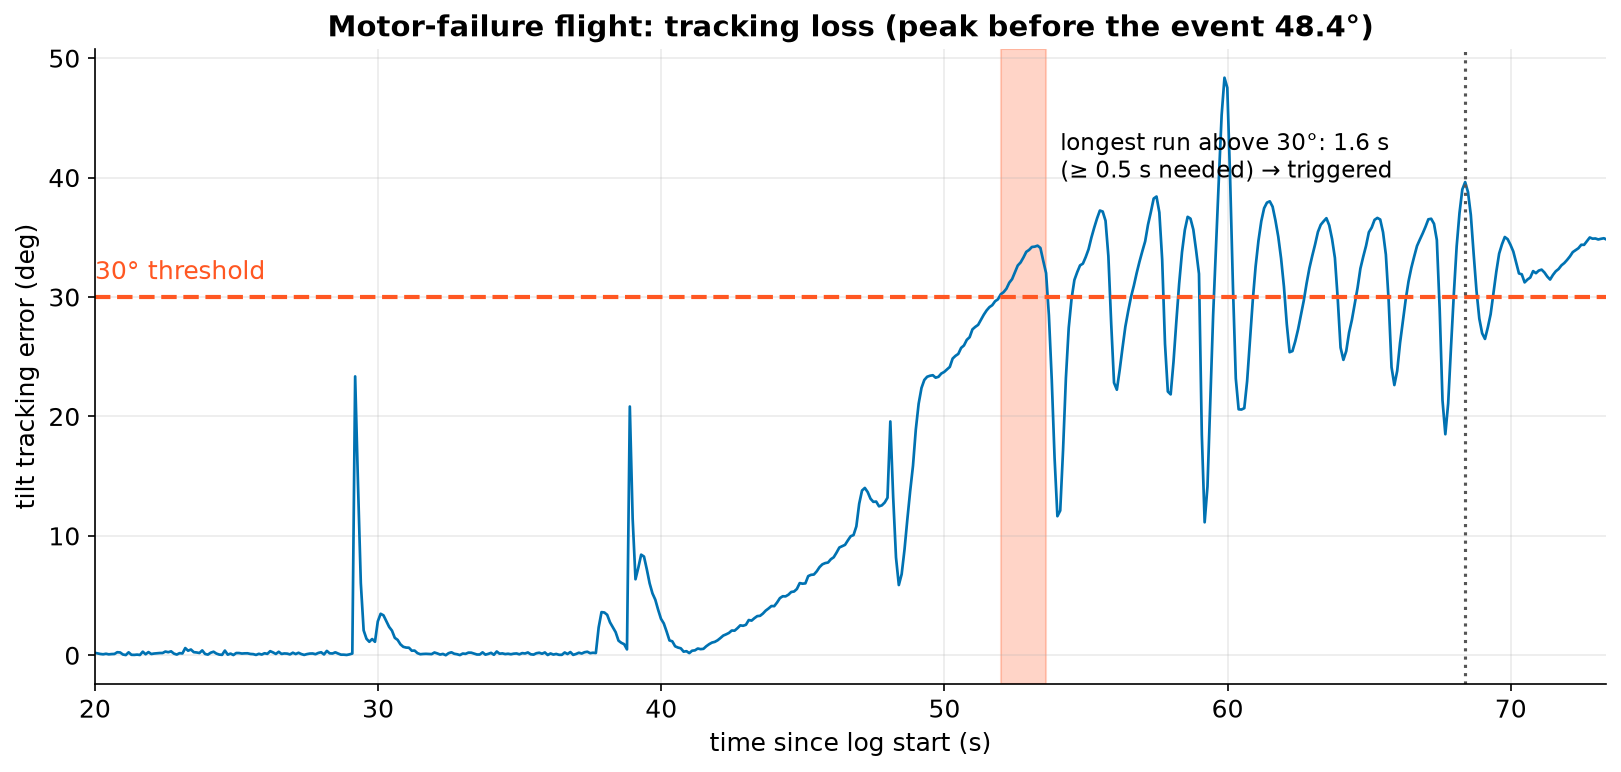
\includegraphics[width=\linewidth,height=0.42\textheight,keepaspectratio]{images/guide/14_tilt_error_timeseries.png}
\caption{Tilt error over time}
\end{figure}

In the nominal flight the tilt error never exceeds \textbf{23.4\textdegree{}}, during brisk turns. In the motor-failure flight it
first passes 30\textdegree{} at \textbf{51.99 s} and peaks at \textbf{48.4\textdegree{}} before the event window ends. The longest stretch above 30\textdegree{}
lasts \textbf{1.6 s}. The \texttt{tracking-loss} rule needs \textbf{30\textdegree{} for at least 0.5 s}, so it is \textbf{triggered}.

\begin{guidebox}{Tilt error is a symptom, not a cause}{orange!80!black}
A large tilt error says ``the drone could not do what it was told''. It doesn't say why. A weak motor, a loose
prop, the wrong frame type, a very aggressive tune or a strong gust can all cause it. AnaTele uses it as
evidence for the \emph{thrust/configuration} hypothesis (chapter 9), together with the motor signals in chapter 6.
\end{guidebox}
\chapter{Motors and mixing}
\label{ch:06-motors-and-mixing}

\section{The mixer}

The pilot or autopilot asks for four things: \textbf{throttle} (up/down), \textbf{roll}, \textbf{pitch} and \textbf{yaw}. The
\textbf{mixer} turns these into one command per motor.

\begin{figure}[H]\centering
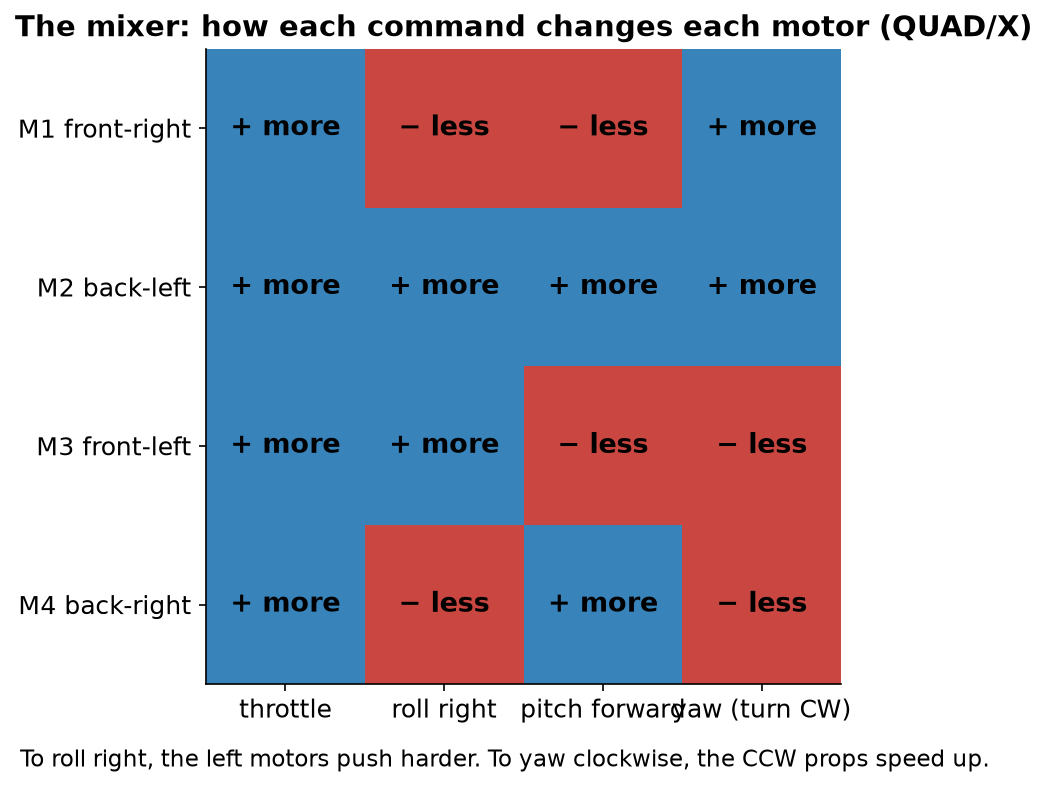
\includegraphics[width=\linewidth,height=0.42\textheight,keepaspectratio]{images/guide/17_mixer_matrix.png}
\caption{Mixer matrix}
\end{figure}

For each motor at arm position $(x, y)$ (right, forward) with spin $s$ (+1 for CCW, $-$1 for CW), the command is
roughly

\[
 u_i = \text{throttle} \;-\; x_i\,\text{roll} \;+\; y_i\,\text{pitch} \;+\; s_i\,\text{yaw}. 
\]

Each command must stay between \texttt{MOT\_\allowbreak{}SPIN\_\allowbreak{}MIN} and \texttt{MOT\_\allowbreak{}SPIN\_\allowbreak{}MAX}. If the sum doesn't fit, ArduPilot (and
AnaTele's simulator) keeps roll and pitch, because they keep the drone upright, and gives up yaw first.

Try it: push the roll slider until one motor hits a limit.

\begin{guidebox}{Interactive}{gray!60!black}This page has an interactive \emph{mixer} widget in the web version: \url{https://avinashistoocool.github.io/AnaTele/learn/06-motors-and-mixing/}\end{guidebox}

\section{Healthy motors}

\begin{figure}[H]\centering
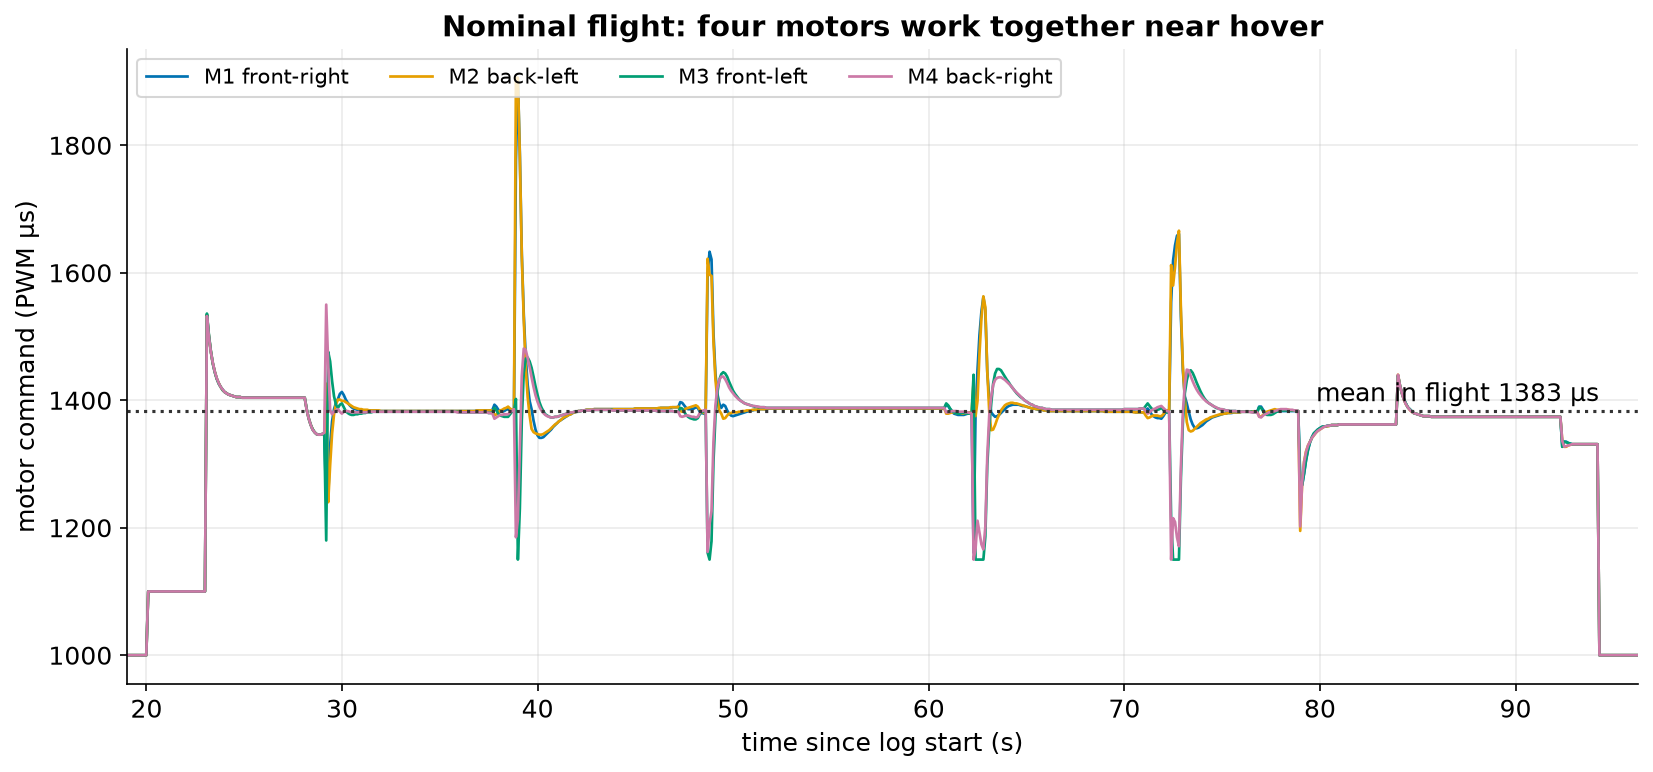
\includegraphics[width=\linewidth,height=0.42\textheight,keepaspectratio]{images/guide/15_motor_outputs_nominal.png}
\caption{Nominal motor outputs}
\end{figure}

In the nominal flight all four commands move together around a mean of about \textbf{1383 \textmu{}s} while airborne.
They spread apart briefly in turns and accelerations.

\section{A failing motor}

In the motor-failure scenario, the simulator makes motor 3 lose thrust. Its health falls as
$h_3 = \max(0.3,\; 1 - 0.06\,(t - t_f))$ from $t_f = 40.85$ s. The autopilot doesn't know this. It only sees the
drone tilting the wrong way, so it \textbf{commands motor 3 harder} and the opposite motor (4) softer.

\begin{figure}[H]\centering
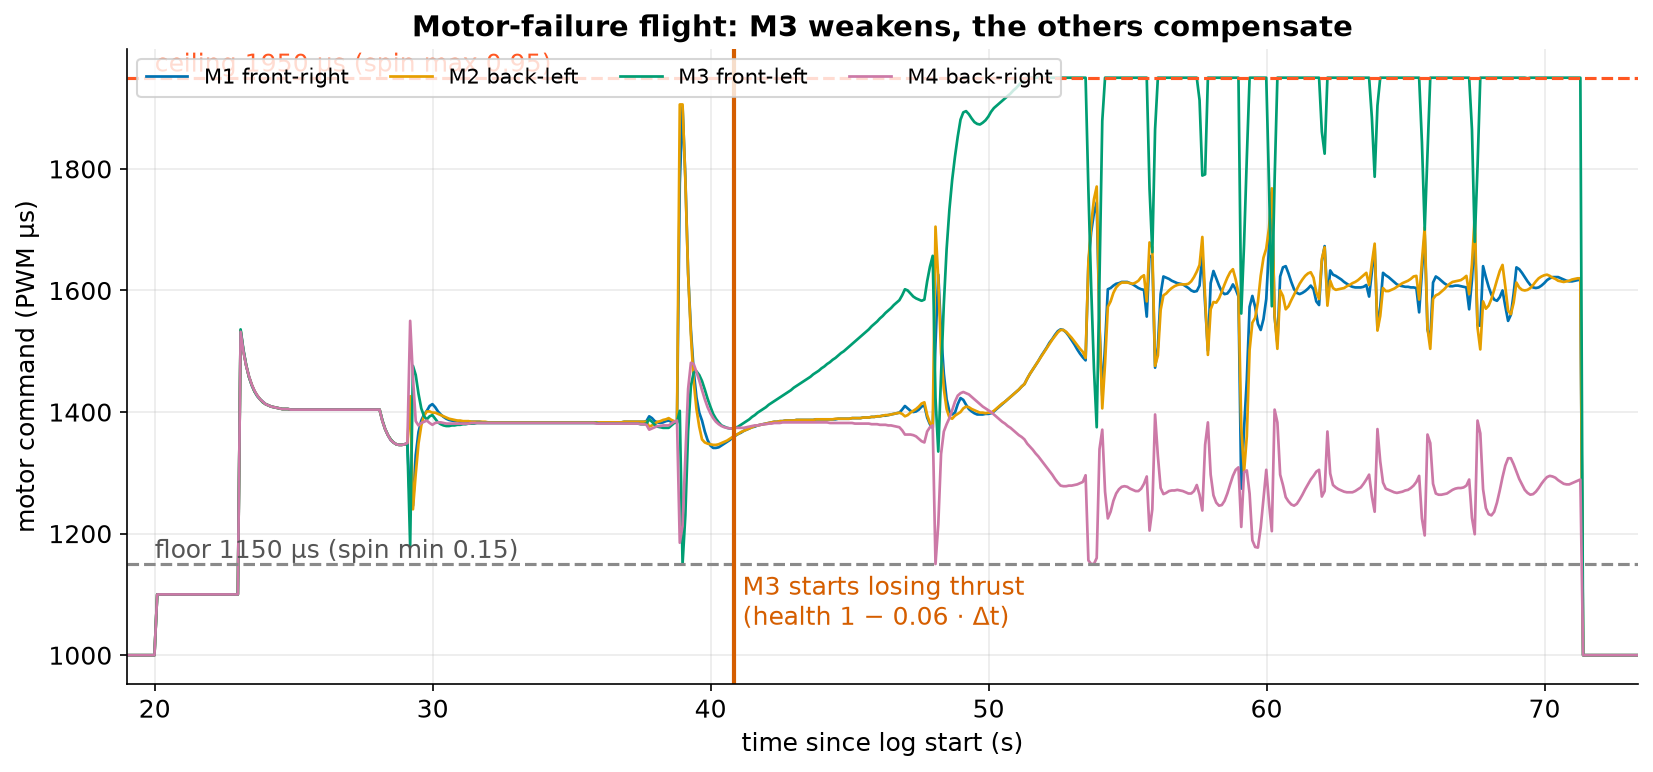
\includegraphics[width=\linewidth,height=0.42\textheight,keepaspectratio]{images/guide/16_motor_outputs_failure.png}
\caption{Motor outputs in failure}
\end{figure}

\begin{guidebox}{Read this the right way round}{green!40!black}
The motor with the \textbf{highest} command is often the \textbf{weak} one. The controller is trying to make up for
missing thrust. A log records \emph{commands}, not thrust, so AnaTele says ``command anomaly'', never ``motor 3 failed''.

\end{guidebox}
\section{Saturation}

A motor is \textbf{at ceiling} if its PWM is within 2 \textmu{}s of the ceiling, and \textbf{at floor} if within 2 \textmu{}s of the floor.
The limits come from the log's own parameters:

\[
 \text{floor} = \text{PWM}_\text{min} + \text{SPIN}_\text{min}\,(\text{PWM}_\text{max} - \text{PWM}_\text{min}) 
\]

\[
 \text{ceiling} = \text{PWM}_\text{min} + \text{SPIN}_\text{max}\,(\text{PWM}_\text{max} - \text{PWM}_\text{min}) 
\]

With 1000--2000 \textmu{}s and spin limits 0.15/0.95, that's \textbf{1150 \textmu{}s} and \textbf{1950 \textmu{}s}.

\begin{figure}[H]\centering
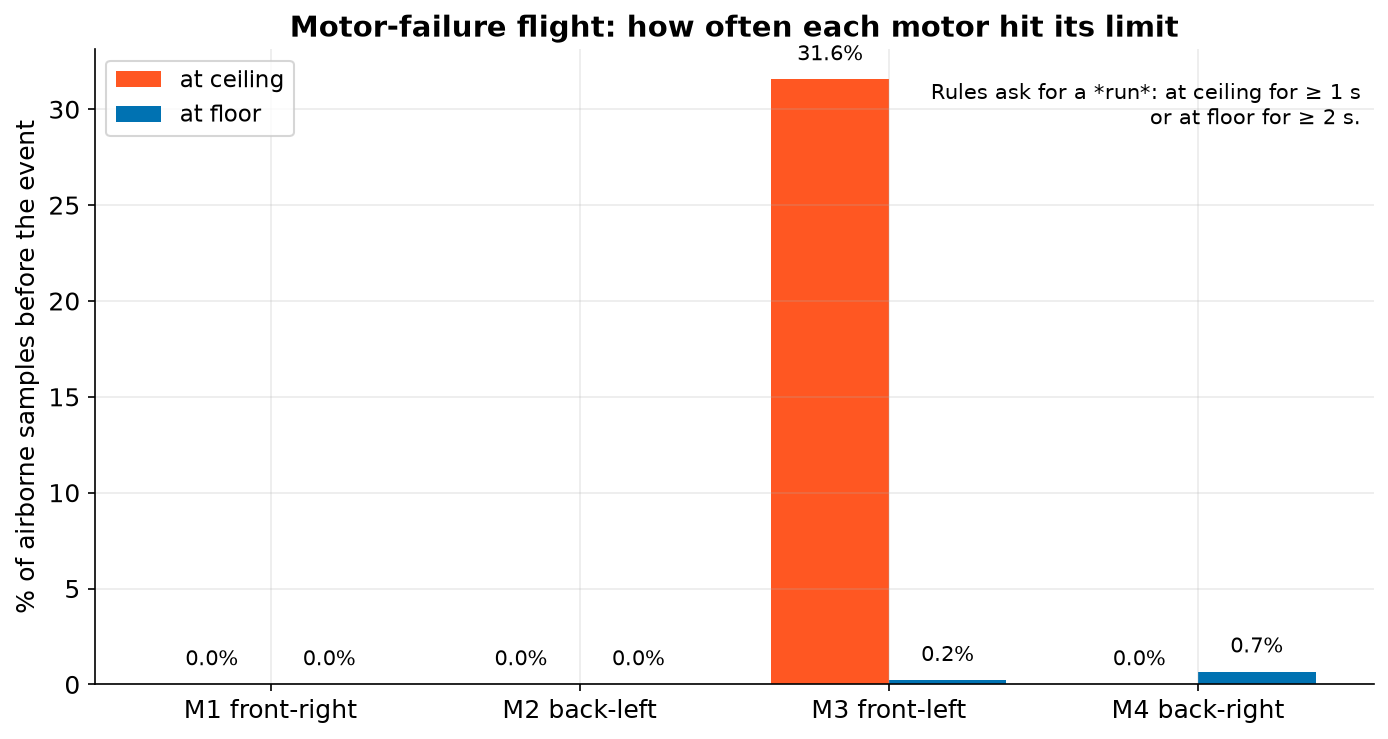
\includegraphics[width=\linewidth,height=0.42\textheight,keepaspectratio]{images/guide/18_saturation_fraction.png}
\caption{Saturation fractions}
\end{figure}

Before the event, motor 3 spends \textbf{31.6 \%} of the airborne samples at its ceiling. Its longest unbroken stretch
is \textbf{2.2 s}. The \texttt{motor-ceiling-saturation} rule needs at least 1 s, so it's \textbf{triggered}. No motor stays at the
floor for 2 s, so \texttt{motor-floor-saturation-pre-event} is not triggered.

\section{Imbalance}

AnaTele also averages each motor's command over the pre-event window (as a fraction of the PWM range). In the
failure flight the means are M1 0.47, M2 0.47, \textbf{M3 0.65}, \textbf{M4 0.34}: a spread of \textbf{0.31}, above the 0.12
screening limit. \texttt{motor-output-imbalance-pre-event} is triggered. Wind, payload offset and yaw demand can also cause
imbalance, and the report says so.
\chapter{Vibration, EKF and compass}
\label{ch:07-vibration-ekf-compass}

\section{Vibration}

The accelerometers measure acceleration, which the autopilot needs to know which way is down. A damaged propeller,
loose motor or stiff mounting adds shaking that the accelerometers also pick up. Too much of it and the position
and altitude estimates degrade.

ArduPilot logs vibration levels in m/s\textsuperscript{2} for each axis. Its own guidance treats \textbf{30} as worth looking at and \textbf{60}
as bad.

\begin{figure}[H]\centering
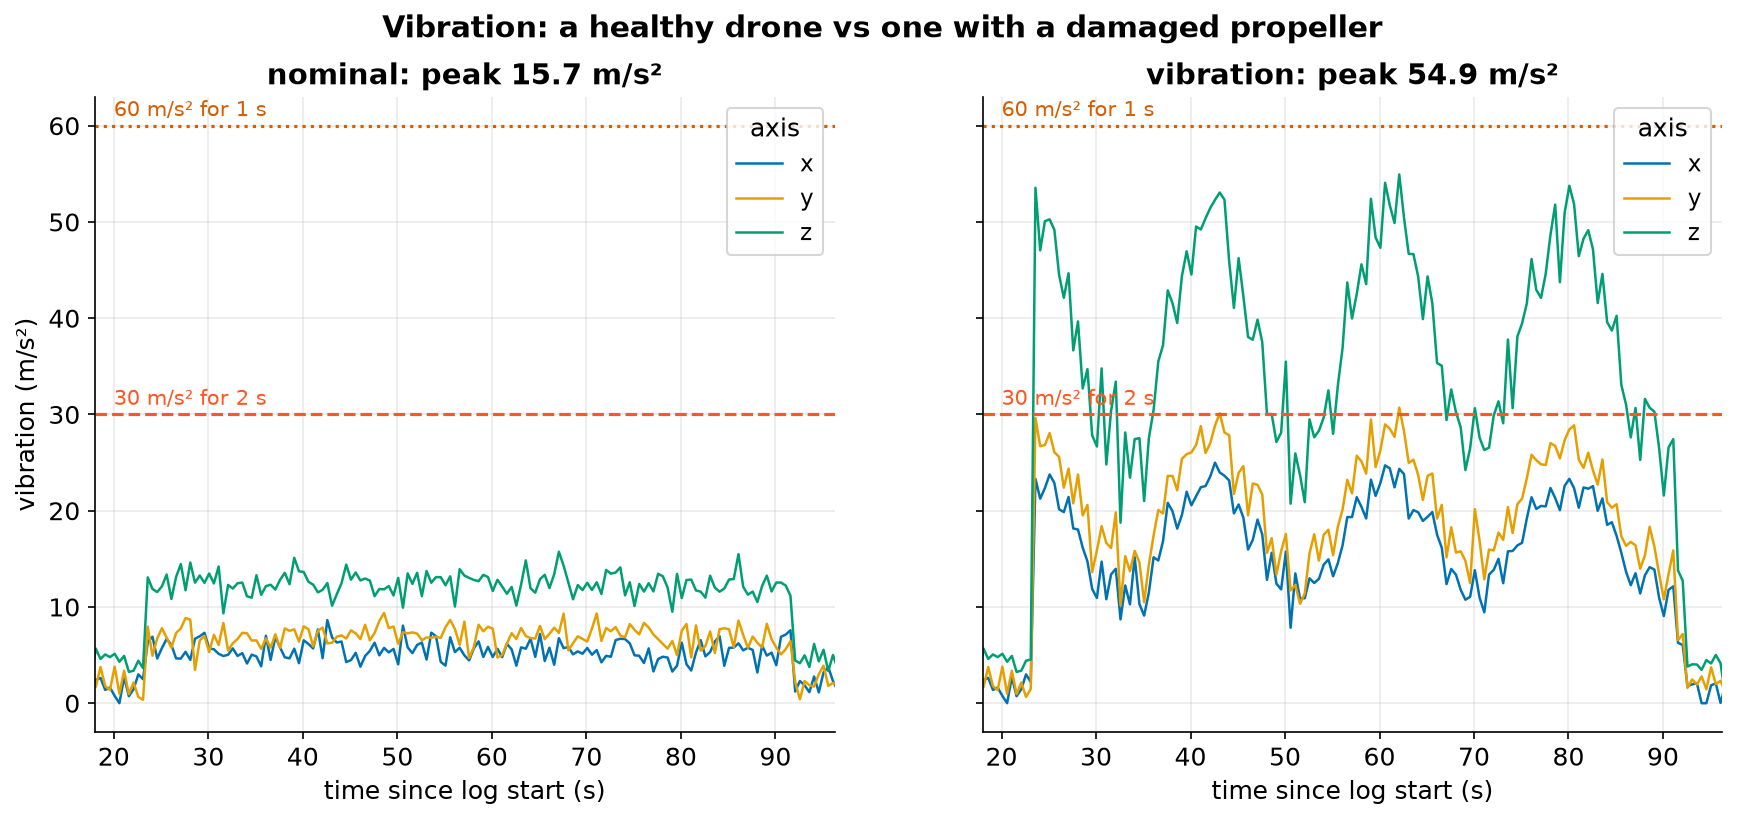
\includegraphics[width=\linewidth,height=0.42\textheight,keepaspectratio]{images/guide/19_vibration_nominal_vs_bad.png}
\caption{Vibration comparison}
\end{figure}

\begin{center}\small
\begin{tabularx}{\linewidth}{XXXX}
\toprule
Flight & Peak vibration & Longest run above 30 m/s\textsuperscript{2} (pre-event) & Rule \\
\midrule
nominal & 15.7 m/s\textsuperscript{2} & 0 s & not triggered \\
vibration (damaged prop) & 54.9 m/s\textsuperscript{2} & \textbf{12.5 s} on z & \textbf{triggered} \\
\bottomrule
\end{tabularx}
\end{center}

\texttt{vibration-persistent-pre-event} triggers if any axis stays above \textbf{30 for 2 s} or above \textbf{60 for 1 s}. The
damaged-prop flight also logged \textbf{283 accelerometer clipping events}, where the sensor hit its maximum, so
\texttt{clipping-pre-event} triggers too.

\section{The EKF: the autopilot's best guess}

ArduPilot fuses all its sensors in an \textbf{Extended Kalman Filter (EKF)}. For each sensor it predicts what the next
reading should be, then compares that with the actual reading. The gap, scaled by how big a gap it expects, is
the \textbf{test ratio}:

\[
 \text{ratio} = \frac{\text{innovation}^2}{\text{expected variance}} \quad\text{(reported so that } 1.0 = \text{at the limit).} 
\]

Below 1 means the sensor agrees with the filter. Above 1 means the EKF is starting to distrust it.

\section{Compass interference}

High motor currents create magnetic fields. If the compass sits too close to the power wires, its heading shifts
whenever the motors work hard.

\begin{figure}[H]\centering
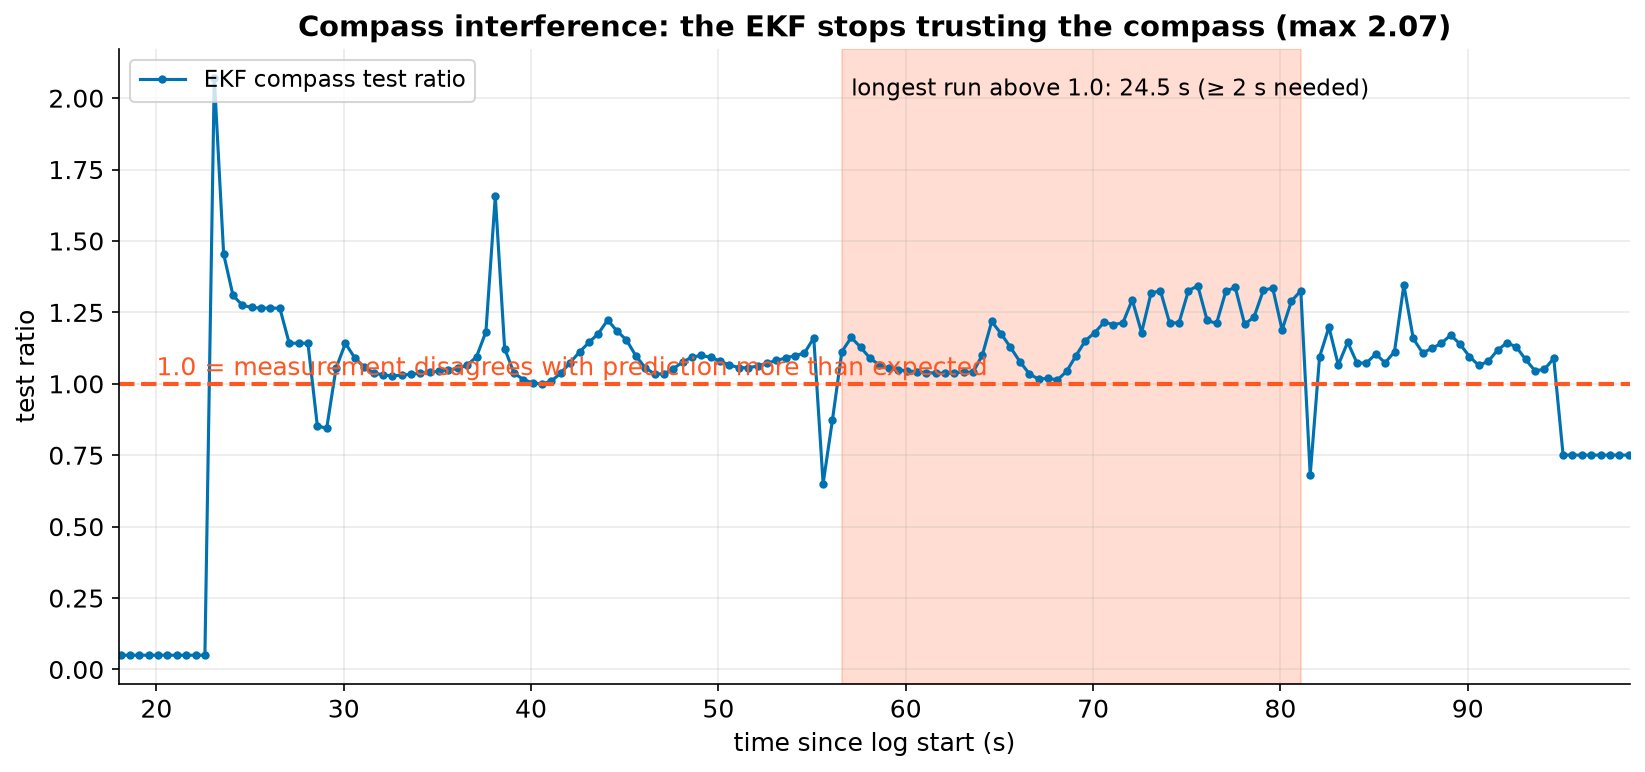
\includegraphics[width=\linewidth,height=0.42\textheight,keepaspectratio]{images/guide/20_ekf_compass_ratio.png}
\caption{EKF compass ratio}
\end{figure}

In the compass-interference flight, the EKF compass ratio reached \textbf{2.07}. Before the event it stayed above 1.0 for
\textbf{24.5 s} in one run. \texttt{ekf-compass-innovation-pre-event} needs \textbf{above 1.0 for 2 s}, so it's \textbf{triggered}.

\begin{figure}[H]\centering
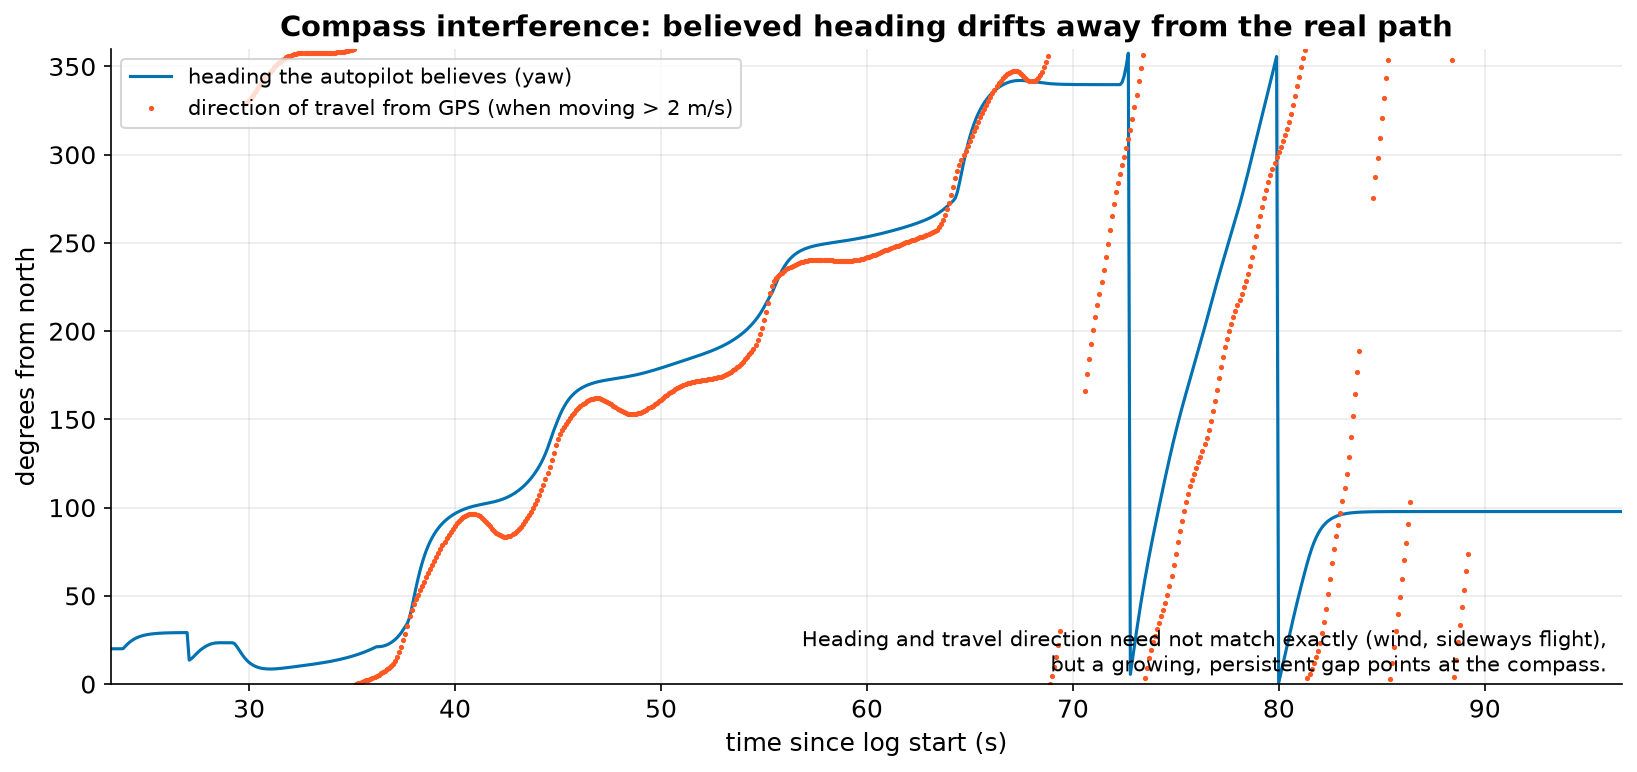
\includegraphics[width=\linewidth,height=0.42\textheight,keepaspectratio]{images/guide/21_heading_disagreement.png}
\caption{Heading disagreement}
\end{figure}

When the heading is wrong, the drone flies in curving, growing circles (``toilet-bowling''). The autopilot steers
for where it \emph{thinks} it's facing, not where it actually is.

\begin{guidebox}{Why a 'compasses inconsistent' message after a crash proves little}{blue!50!black}
After the motor-failure crash, the simulator (like real ArduPilot) printed \emph{``PreArm: Compasses inconsistent''}.
A crash can bend a compass mount, so this message comes \emph{after} the incident. AnaTele records it
(\texttt{compasses-inconsistent-reported}) but gives it little weight.
\end{guidebox}
\chapter{Rules and their four states}
\label{ch:08-rules-and-states}

\section{What a rule is}

A rule is a small, versioned, written-down check: "if \emph{this signal} stays above \emph{this threshold} for \emph{this long},
during \emph{this phase}, report it". All rules live in one file, the \textbf{rule pack} (\texttt{telemetry\_\allowbreak{}platform/rules/core.yaml}).
Every report records which pack version and SHA-256 it used, so the same log always gives the same answer.

\section{Persistence: ignore blips, catch trends}

\begin{figure}[H]\centering
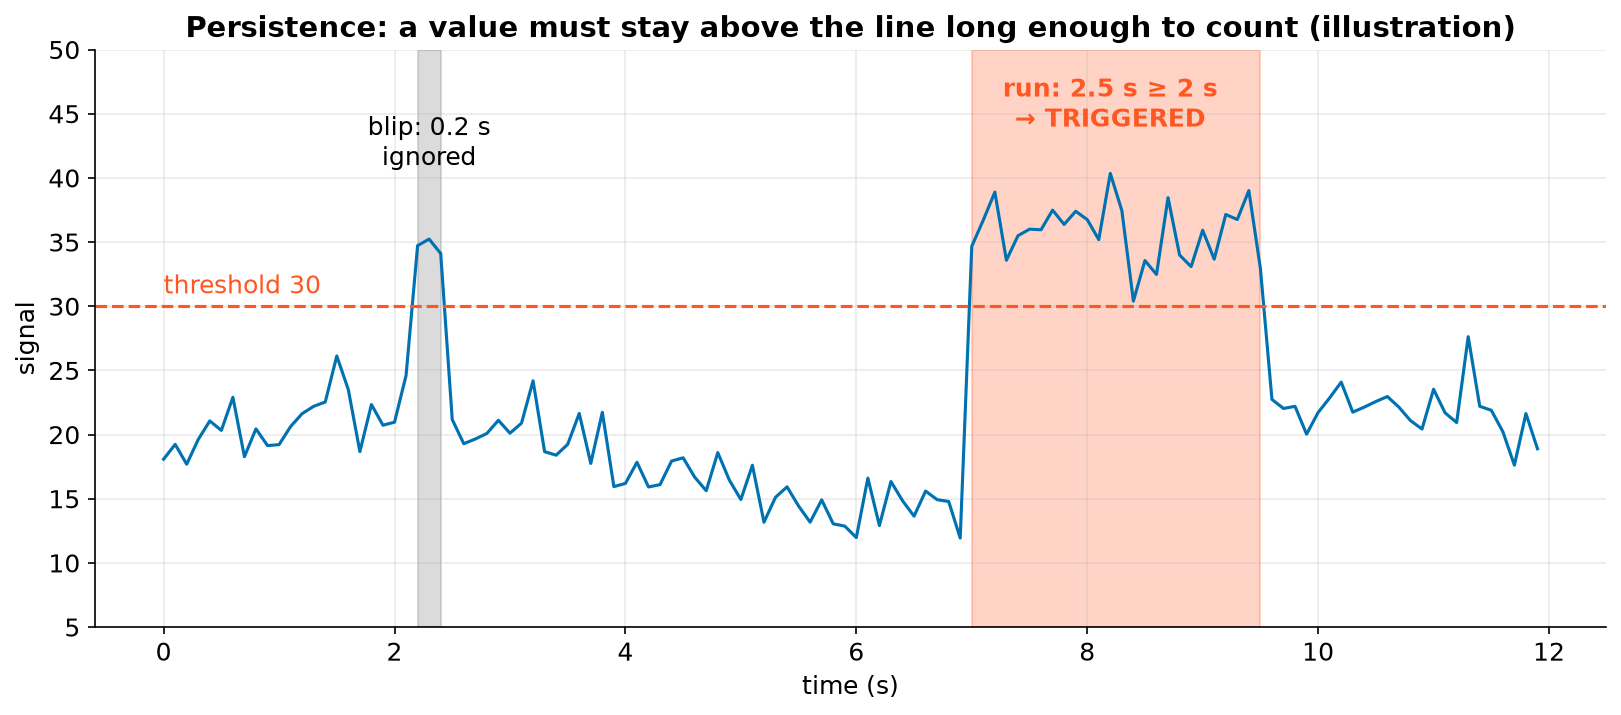
\includegraphics[width=\linewidth,height=0.42\textheight,keepaspectratio]{images/guide/22_persistence_rule.png}
\caption{Persistence}
\end{figure}

Real signals are noisy. A single spike is usually meaningless, so most rules need a \textbf{run}: consecutive samples
above the threshold, lasting at least \texttt{for\_\allowbreak{}s} seconds. Two more details:

\begin{itemize}
\item If two samples are too far apart (more than the \textbf{maximum gap}), the run is broken. AnaTele doesn't assume what
happened in between.
\item A run's length is measured from its \textbf{first to its last} sample above the threshold.
\end{itemize}

Try it, including what happens when data gets sparse:

\begin{guidebox}{Interactive}{gray!60!black}This page has an interactive \emph{persistence} widget in the web version: \url{https://avinashistoocool.github.io/AnaTele/learn/08-rules-and-states/}\end{guidebox}

\section{The four states}

\begin{figure}[H]\centering
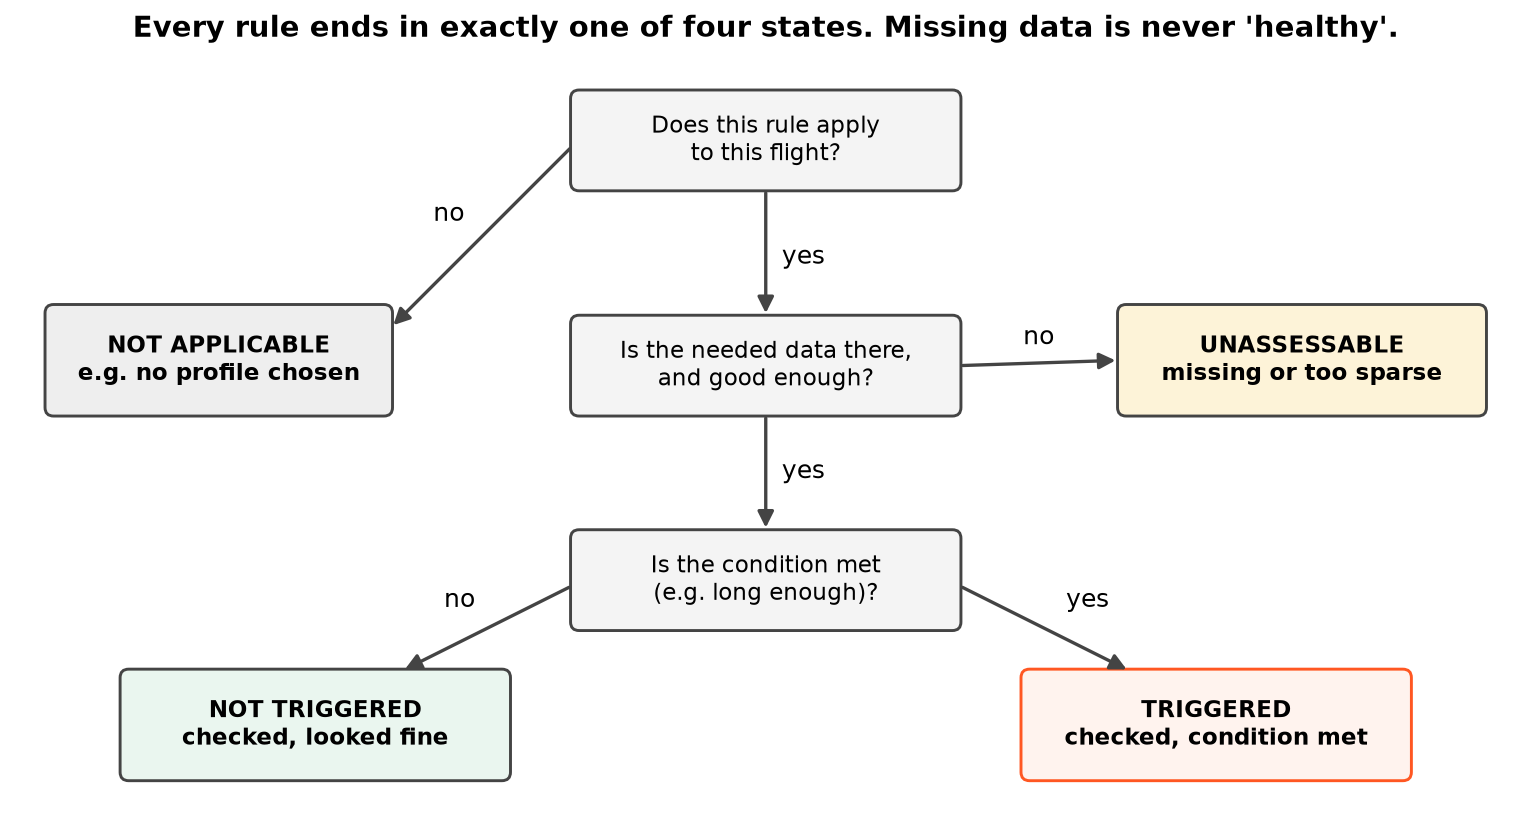
\includegraphics[width=\linewidth,height=0.42\textheight,keepaspectratio]{images/guide/23_rule_states.png}
\caption{Rule states flow}
\end{figure}

\begin{center}\small
\begin{tabularx}{\linewidth}{p{0.30\linewidth}X}
\toprule
State & Meaning \\
\midrule
\textbf{triggered} & The data is there and the condition was met. \\
\textbf{not triggered} & The data is there and the condition was \emph{not} met. \\
\textbf{unassessable} & The data needed is missing, or too sparse to decide. \textbf{Not the same as healthy.} \\
\textbf{not applicable} & The rule doesn't apply here, e.g. a profile check when no profile was selected. \\
\bottomrule
\end{tabularx}
\end{center}

Here are real examples from the simulated flights:

\begin{figure}[H]\centering
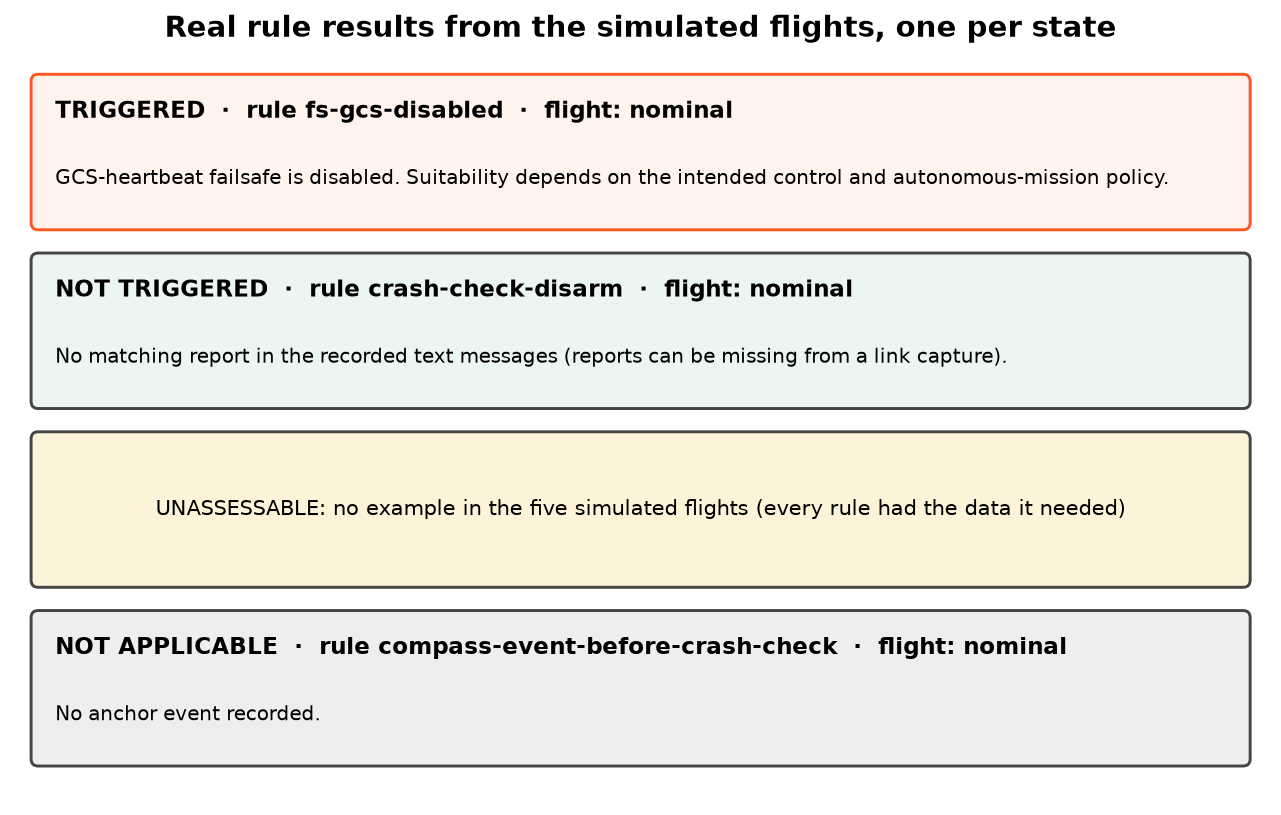
\includegraphics[width=\linewidth,height=0.42\textheight,keepaspectratio]{images/guide/32_four_states_examples.png}
\caption{Four states examples}
\end{figure}

\begin{guidebox}{Unknown is never healthy}{orange!80!black}
Many tools show a green tick when a check \emph{couldn't run}. AnaTele never does. If a log has no vibration data,
the vibration rules say \textbf{unassessable}, and any hypothesis that depends on them says so too.

\end{guidebox}
\section{Counting the five simulated flights}

\begin{center}\small
\begin{tabularx}{\linewidth}{XXXX}
\toprule
Flight & triggered & not triggered & not applicable \\
\midrule
nominal & 1 & 19 & 2 \\
motor\_failure & 7 & 14 & 1 \\
compass\_interference & 2 & 18 & 2 \\
vibration & 5 & 15 & 2 \\
radio\_failsafe & 2 & 18 & 2 \\
\bottomrule
\end{tabularx}
\end{center}

The one rule that triggers even in the nominal flight is \texttt{fs-gcs-disabled}. It's a configuration observation
(the ground-station failsafe is turned off), not a fault. That's why rules have \textbf{severities} and are kept
separate from \textbf{hypotheses}.
\chapter{Hypotheses}
\label{ch:09-hypotheses}

Rules say \textbf{what was observed}. Hypotheses ask \textbf{what could explain it}. AnaTele ranks the hypotheses only for
episodes that end in a critical event (an autopilot crash report). In the five simulated flights that's only the
motor-failure flight.

\section{The four built-in hypotheses}

\begin{center}\small
\begin{tabularx}{\linewidth}{XXX}
\toprule
Hypothesis & Supported by (family, weight) & Counted against it \\
\midrule
Mechanical / thrust or frame configuration & tracking-loss (control, 1) $\cdot$ motor floor saturation (propulsion, 1) $\cdot$ motor imbalance (propulsion, 0.75) $\cdot$ motor ceiling saturation (propulsion, 0.5) & -- \\
Estimator / magnetic inconsistency & compass event before crash check (estimator, 1) $\cdot$ EKF compass innovation (magnetic, 1) $\cdot$ compasses inconsistent reported (magnetic, 0.25) & compass event flagged as coming after the upset (1) \\
Vibration-driven estimation degradation & persistent vibration (inertial, 1) $\cdot$ clipping (inertial, 1) & vibration \emph{checked and fine} (0.5) $\cdot$ clipping \emph{checked and fine} (0.5) \\
Electrical / power degradation & no support rules yet in this pack version & blocked if \texttt{power-monitoring-gap} fires \\
\bottomrule
\end{tabularx}
\end{center}

\section{The score}

\[
 \text{score} = \sum_{\text{families } f} \min\!\Big(1.5,\; \sum_{\text{triggered rules in } f} w\Big) \;-\; \sum_{\text{contradictions}} w 
\]

The \textbf{family cap of 1.5} matters. Three rules that all measure motor commands are not three independent pieces of
evidence. Capping each family stops one kind of evidence from dominating. Evidence from \textbf{different} families
(say, \emph{control} and \emph{propulsion}) does add up.

\begin{center}\small
\begin{tabularx}{\linewidth}{p{0.30\linewidth}X}
\toprule
Label & When \\
\midrule
strong support & score $\geq$ 2 \\
some support & score $\geq$ 1 \\
weak support & score > 0 \\
mixed support & there is both support and contradiction \\
limited or contradicting evidence & score $\leq$ 0 \\
unassessable & none of its rules could be checked (or a blocking rule fired) \\
\bottomrule
\end{tabularx}
\end{center}

\section{Worked example: the motor-failure flight}

\begin{figure}[H]\centering
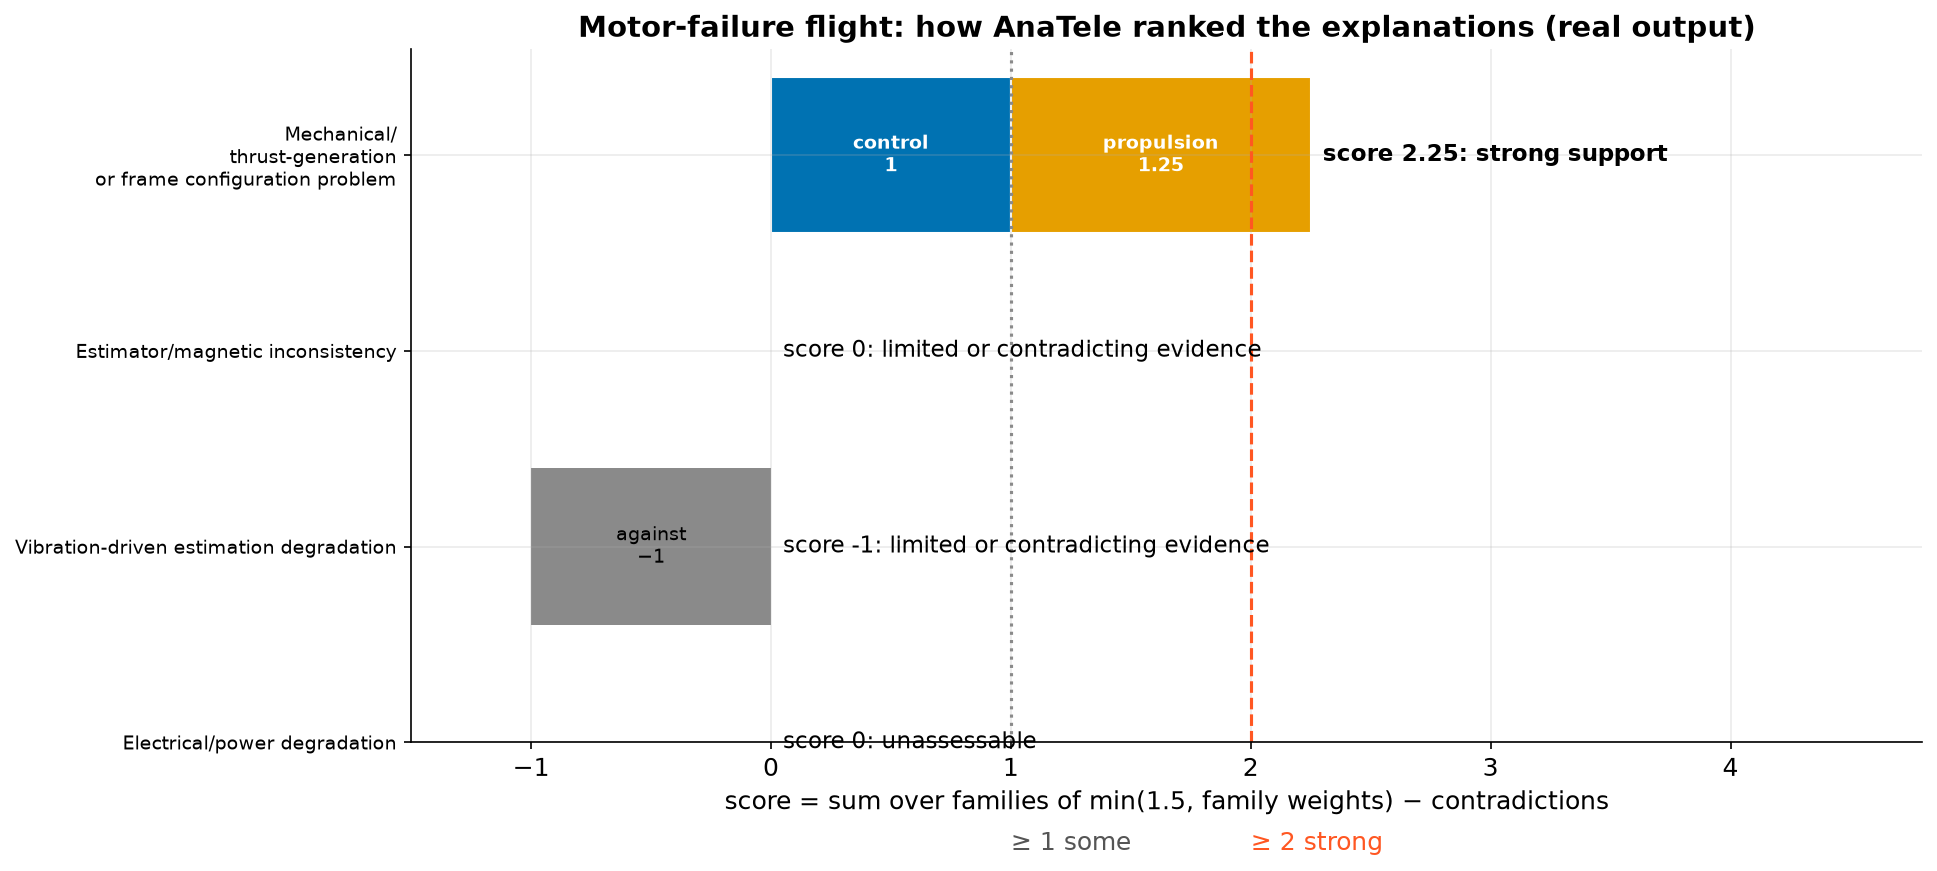
\includegraphics[width=\linewidth,height=0.42\textheight,keepaspectratio]{images/guide/24_hypothesis_scoring.png}
\caption{Hypothesis scoring}
\end{figure}

\begin{itemize}
\item \textbf{Thrust/configuration}: control family = 1 (tracking-loss). Propulsion family = 0.75 + 0.5 = 1.25
(imbalance + ceiling), under the cap. Score = 1 + 1.25 = \textbf{2.25}, so \textbf{strong support}.
\item \textbf{Vibration}: nothing triggered, and both vibration rules were \emph{checked and fine}, giving $-$0.5 $-$ 0.5 =
\textbf{$-$1.0}: \emph{limited or contradicting evidence}. Checking and finding nothing counts \textbf{against} an explanation.
\item \textbf{Magnetic}: score \textbf{0}. The post-crash ``Compasses inconsistent'' message doesn't count, because it isn't from
the flight's own time window.
\item \textbf{Power}: \textbf{unassessable}. The current pack has no rule that can support it, so it's listed as a reminder of
what the log \emph{can't} tell you. Confirming it needs battery voltage/current logs.
\end{itemize}

Toggle the evidence yourself:

\begin{guidebox}{Interactive}{gray!60!black}This page has an interactive \emph{hypothesis} widget in the web version: \url{https://avinashistoocool.github.io/AnaTele/learn/09-hypotheses/}\end{guidebox}

\begin{guidebox}{This is a screening order, not a probability}{red!60!black}
A score of 2.25 doesn't mean ``90 \% likely''. The weights are written-down expert judgements, and the list tells
you \textbf{what to inspect first}. Each hypothesis also lists the \emph{discriminating evidence} that would confirm or
rule it out. For thrust problems that's ESC RPM/current telemetry, a props-off motor test and a physical
inspection.
\end{guidebox}
\chapter{Missions and geometry}
\label{ch:10-missions-and-geometry}

\section{Where did it go?}

An \textbf{AUTO mission} is a list of numbered items, usually waypoints (latitude, longitude, altitude). The ground
station uploads them, the autopilot flies them in order and reports \texttt{MISSION\_\allowbreak{}ITEM\_\allowbreak{}REACHED} as it gets to each one.

AnaTele rebuilds the uploaded plan from the log's own messages. Then, for each waypoint, it checks whether the
drone actually got there.

\begin{figure}[H]\centering
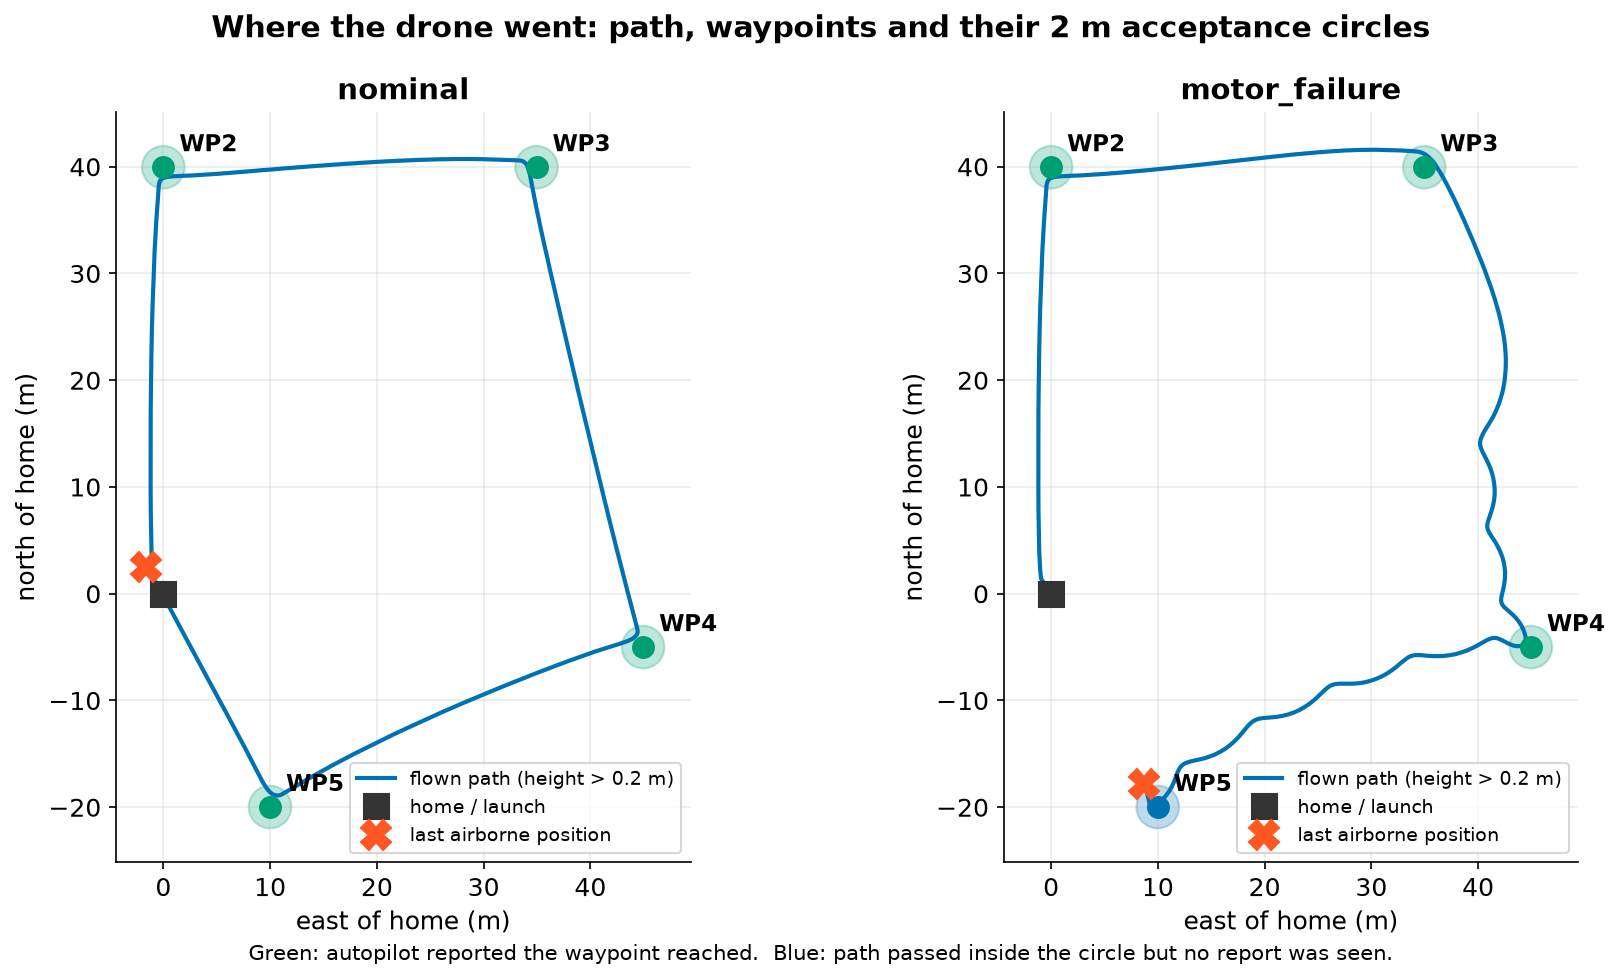
\includegraphics[width=\linewidth,height=0.42\textheight,keepaspectratio]{images/guide/25_mission_map.png}
\caption{Mission map}
\end{figure}

The simulated mission is a takeoff to 10 m, four waypoints and a return-to-launch. In the nominal flight every
waypoint is reported reached. In the motor-failure flight:

\begin{center}\small
\begin{tabularx}{\linewidth}{XXX}
\toprule
Item & Status & Nearest recorded position \\
\midrule
WP2--WP4 & \texttt{reported\_\allowbreak{}complete} & 0.97, 0.97, 0.70 m \\
WP5 & \texttt{geometry\_\allowbreak{}consistent\_\allowbreak{}with\_\allowbreak{}completion} & 0.32 m, but no ``reached'' report before the crash \\
RTL & \texttt{completion\_\allowbreak{}not\_\allowbreak{}observed} & (not a positional item) \\
\bottomrule
\end{tabularx}
\end{center}

\section{Distance on a sphere}

GPS gives latitude and longitude in degrees, but we need metres. On a sphere of radius $R$, the shortest distance
between two points is along the surface. The \textbf{haversine formula} gives it:

\[
 h = \sin^2\!\frac{\Delta\varphi}{2} + \cos\varphi_1 \cos\varphi_2 \sin^2\!\frac{\Delta\lambda}{2}, \qquad d = 2R \arcsin\sqrt{h} 
\]

with $\varphi$ = latitude, $\lambda$ = longitude (in radians) and $R = 6\,371\,008.8$ m (the mean Earth radius).

\begin{figure}[H]\centering
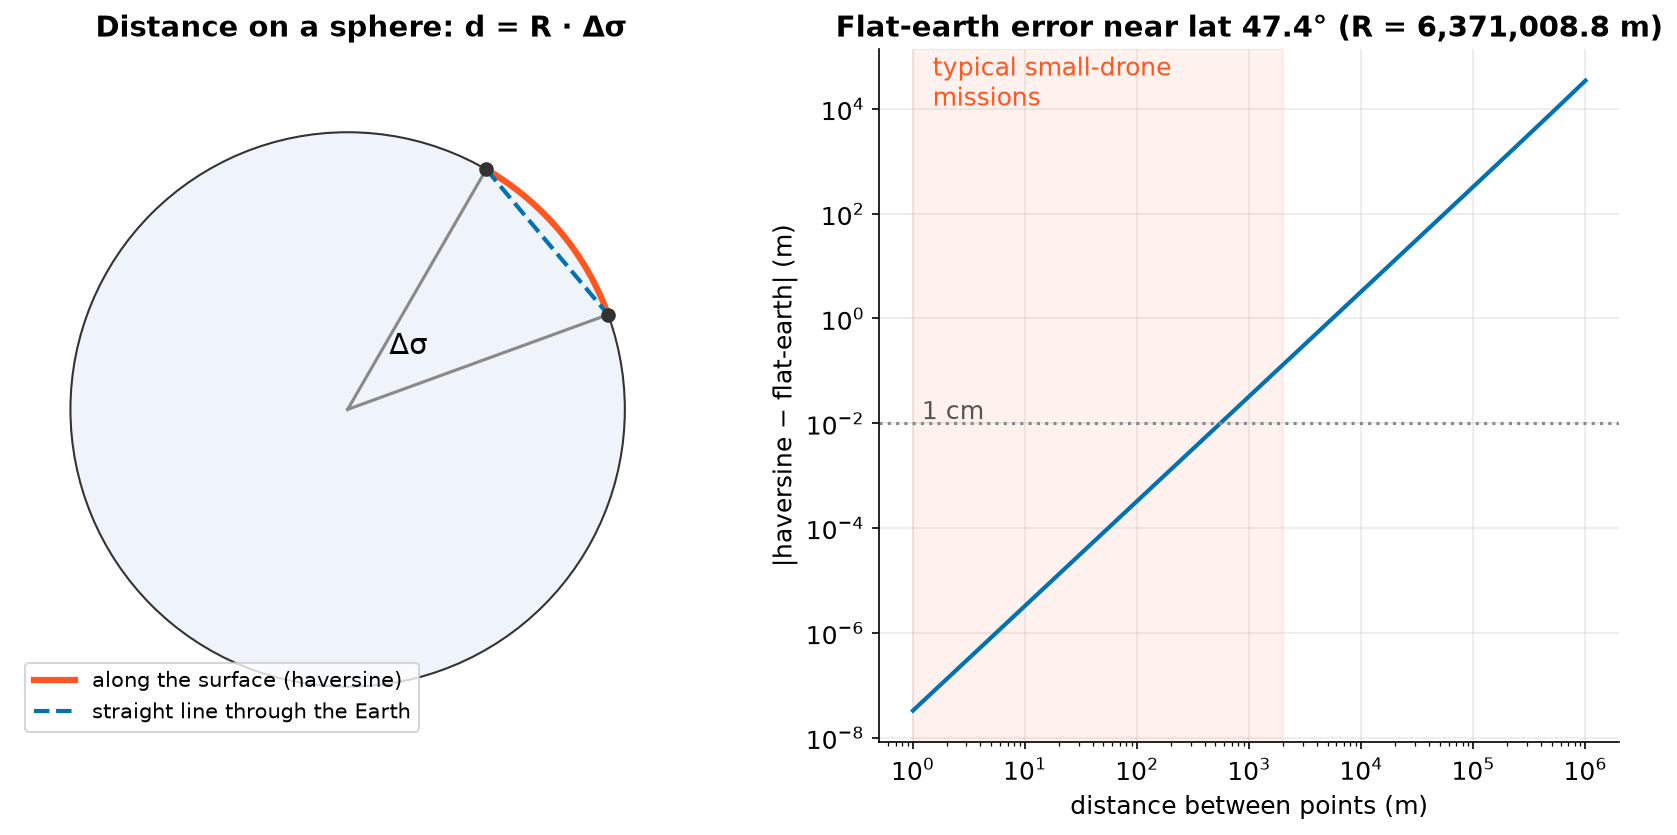
\includegraphics[width=\linewidth,height=0.42\textheight,keepaspectratio]{images/guide/26_haversine.png}
\caption{Haversine}
\end{figure}

Over a few kilometres the flat-earth shortcut is accurate to millimetres, far smaller than GPS error. AnaTele uses
haversine anyway because it's correct everywhere, including long survey flights and high latitudes.

\begin{guidebox}{Interactive}{gray!60!black}This page has an interactive \emph{waypoint} widget in the web version: \url{https://avinashistoocool.github.io/AnaTele/learn/10-missions-and-geometry/}\end{guidebox}

\section{When does a waypoint count as reached?}

ArduPilot treats a waypoint as reached when the drone is within \texttt{WP\_\allowbreak{}RADIUS\_\allowbreak{}M} (2 m in the simulation). GPS has its
own uncertainty, so AnaTele allows

\[
 d_\text{nearest} \le \texttt{WP\_RADIUS\_M} + h_\text{acc} 
\]

where $h_\text{acc}$ is the GPS horizontal accuracy at that moment. Passing this test is labelled *consistent with
completion*, not \emph{completed}: being close isn't proof.

\begin{figure}[H]\centering
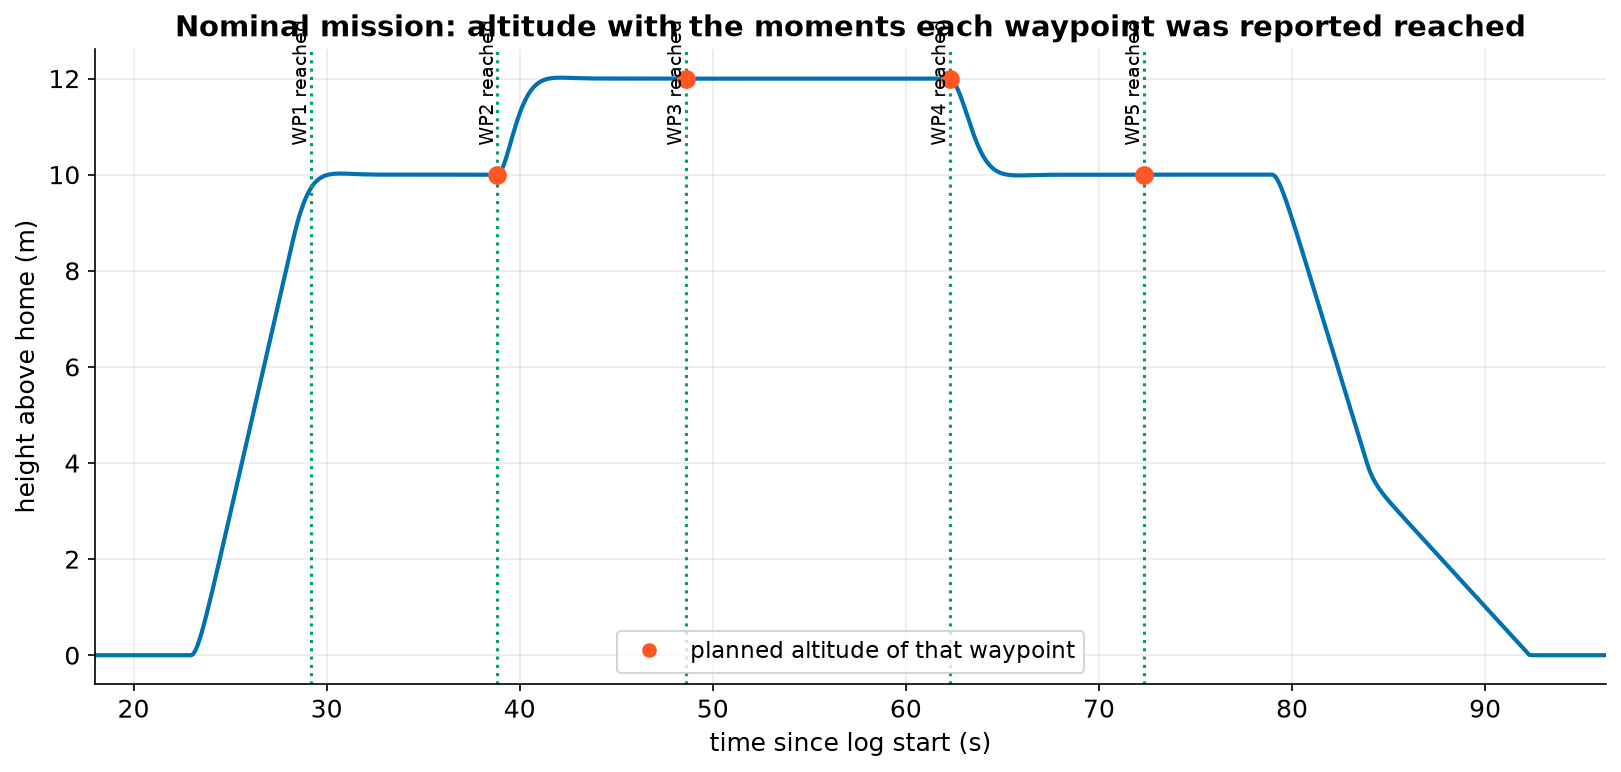
\includegraphics[width=\linewidth,height=0.42\textheight,keepaspectratio]{images/guide/27_altitude_profile_mission.png}
\caption{Altitude profile}
\end{figure}

\section{Drawing the path}

The 3D replay in the desktop app draws the flown path with the waypoints. To keep drawing fast it uses at most
6,000 points, keeping every \emph{k}-th sample with $k = \lceil n / 6000 \rceil$:

\begin{figure}[H]\centering
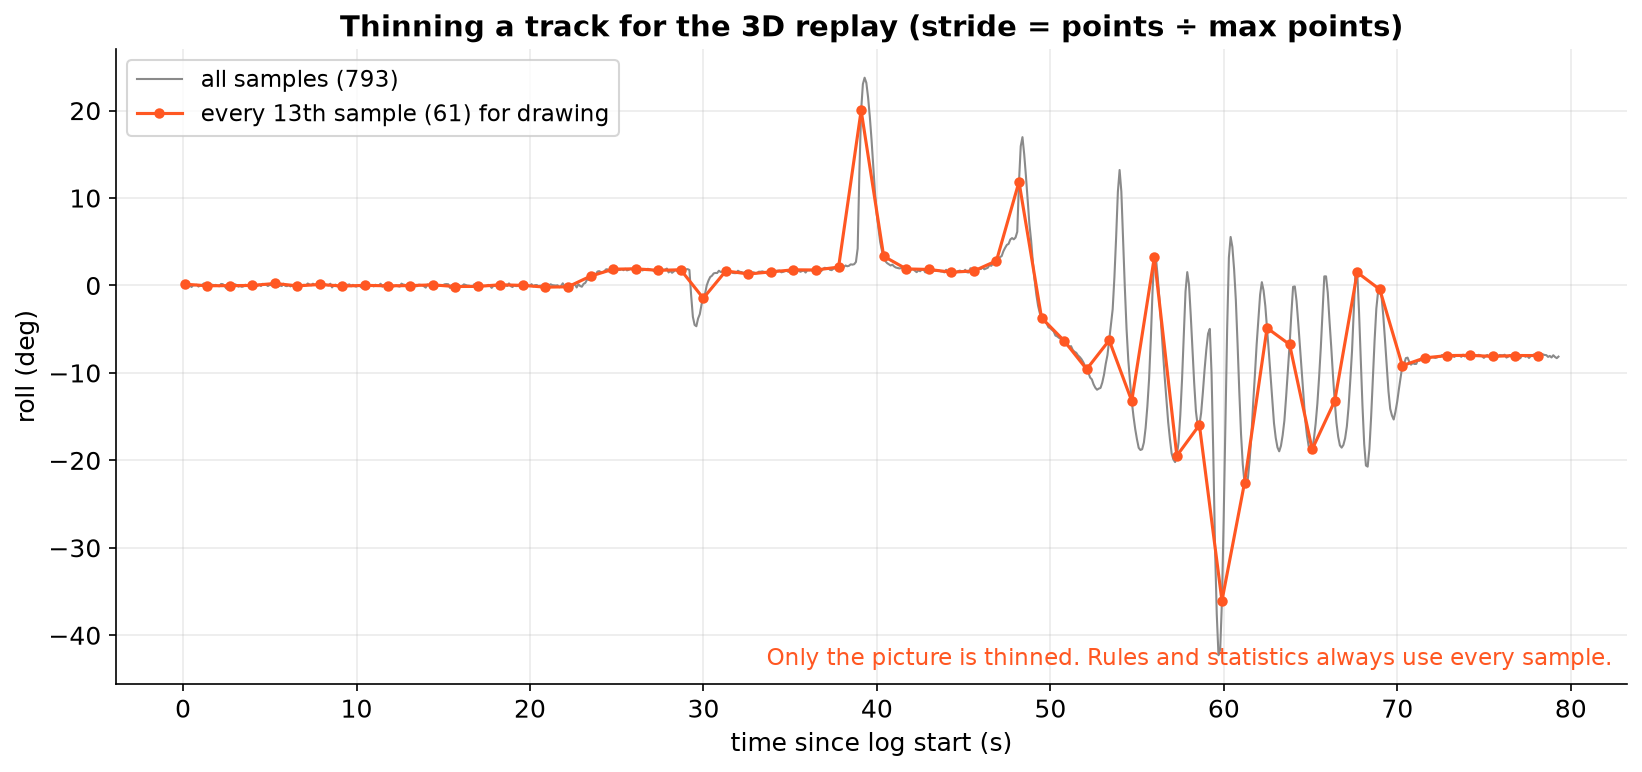
\includegraphics[width=\linewidth,height=0.42\textheight,keepaspectratio]{images/guide/28_downsampling.png}
\caption{Downsampling}
\end{figure}

\begin{guidebox}{Note}{blue!50!black}
Thinning only affects the \textbf{picture}. Every rule, statistic and distance above uses every sample.
\end{guidebox}
\chapter{The simulator}
\label{ch:11-simulator}

Every chart in this course came from AnaTele's built-in flight simulator. It exists so that you can **learn and test
without crashing a real drone**. Each scenario has a known cause, so you can check that the analysis finds it.

\begin{verbatim}
anatele simulate --out simulations          # all five scenarios
anatele simulations/sim_motor_failure.tlog  # analyse one
\end{verbatim}

\section{How it works}

\begin{figure}[H]\centering
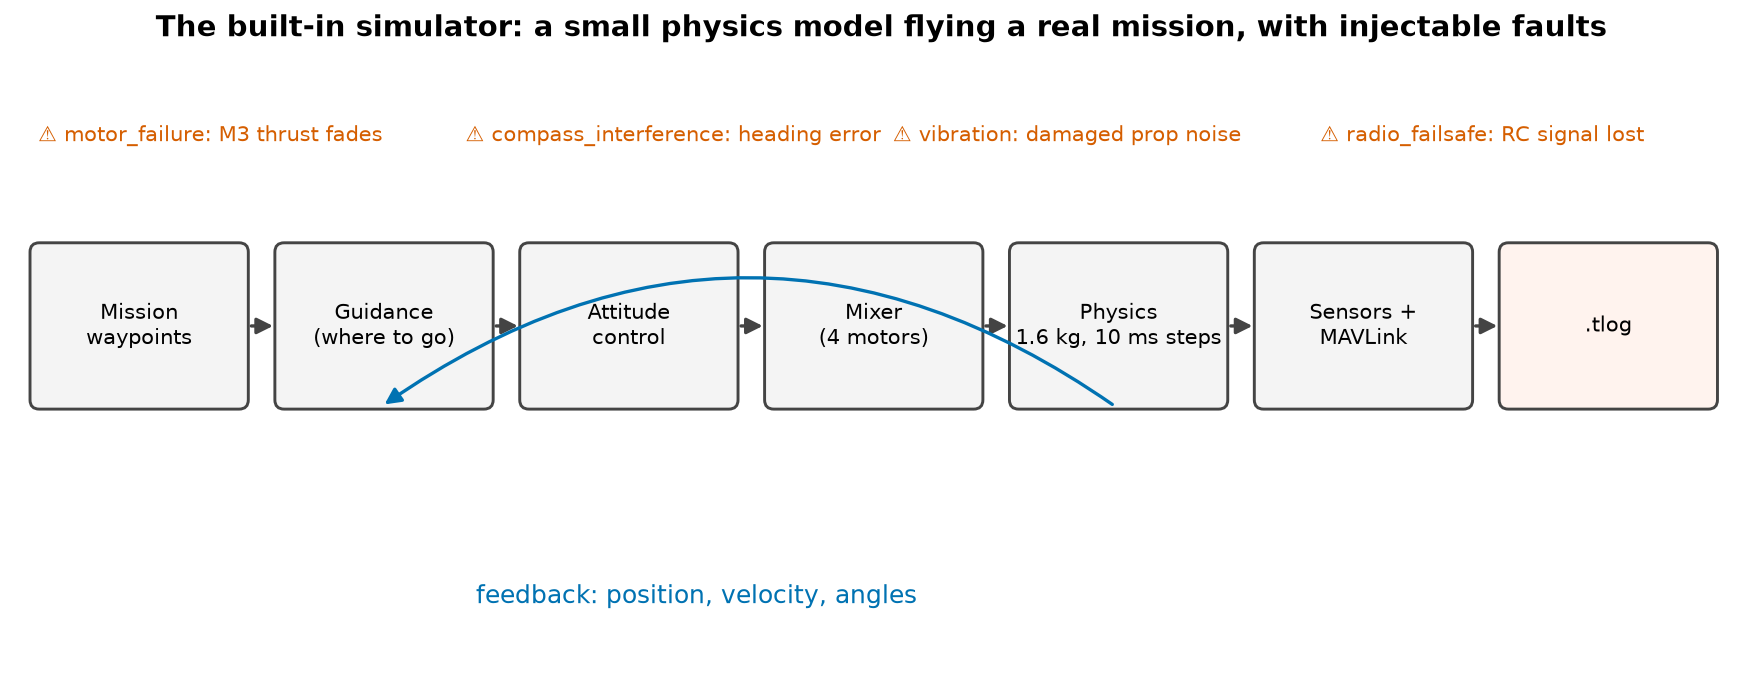
\includegraphics[width=\linewidth,height=0.42\textheight,keepaspectratio]{images/guide/29_simulator_block.png}
\caption{Simulator block diagram}
\end{figure}

Every \textbf{10 ms} the simulator:

\begin{enumerate}
\item \textbf{Guidance} picks a target velocity towards the active waypoint.
\item \textbf{Attitude control} turns that into desired roll and pitch (capped at 0.52 rad $\approx$ 30\textdegree{}), and a yaw target.
\item The \textbf{mixer} (chapter 6) turns throttle and torques into four motor commands between 0.15 and 0.95.
\item \textbf{Physics} turns commands into thrust and torque. It then integrates Newton's laws for a 1.6 kg quad with
0.18 m arms, drag and a gusting wind.
\item \textbf{Sensors and MAVLink}: every 100 ms it writes \texttt{ATTITUDE}, \texttt{GLOBAL\_\allowbreak{}POSITION\_\allowbreak{}INT}, \texttt{SERVO\_\allowbreak{}OUTPUT\_\allowbreak{}RAW} and
more (and slower health messages every 500 ms) into a genuine \texttt{.tlog}, byte for byte as Mission Planner would.
\end{enumerate}

The thrust per motor is

\[
 F_i = h_i \cdot F_\text{max} \cdot u_i, \qquad F_\text{max} = \frac{m g}{4 \cdot 0.38} \approx 10.3\ \text{N}, 
\]

so at the hover output 0.38, four healthy motors exactly hold the weight. $h_i$ is the motor's \textbf{health} (1 =
perfect).

\section{The five scenarios}

\begin{figure}[H]\centering
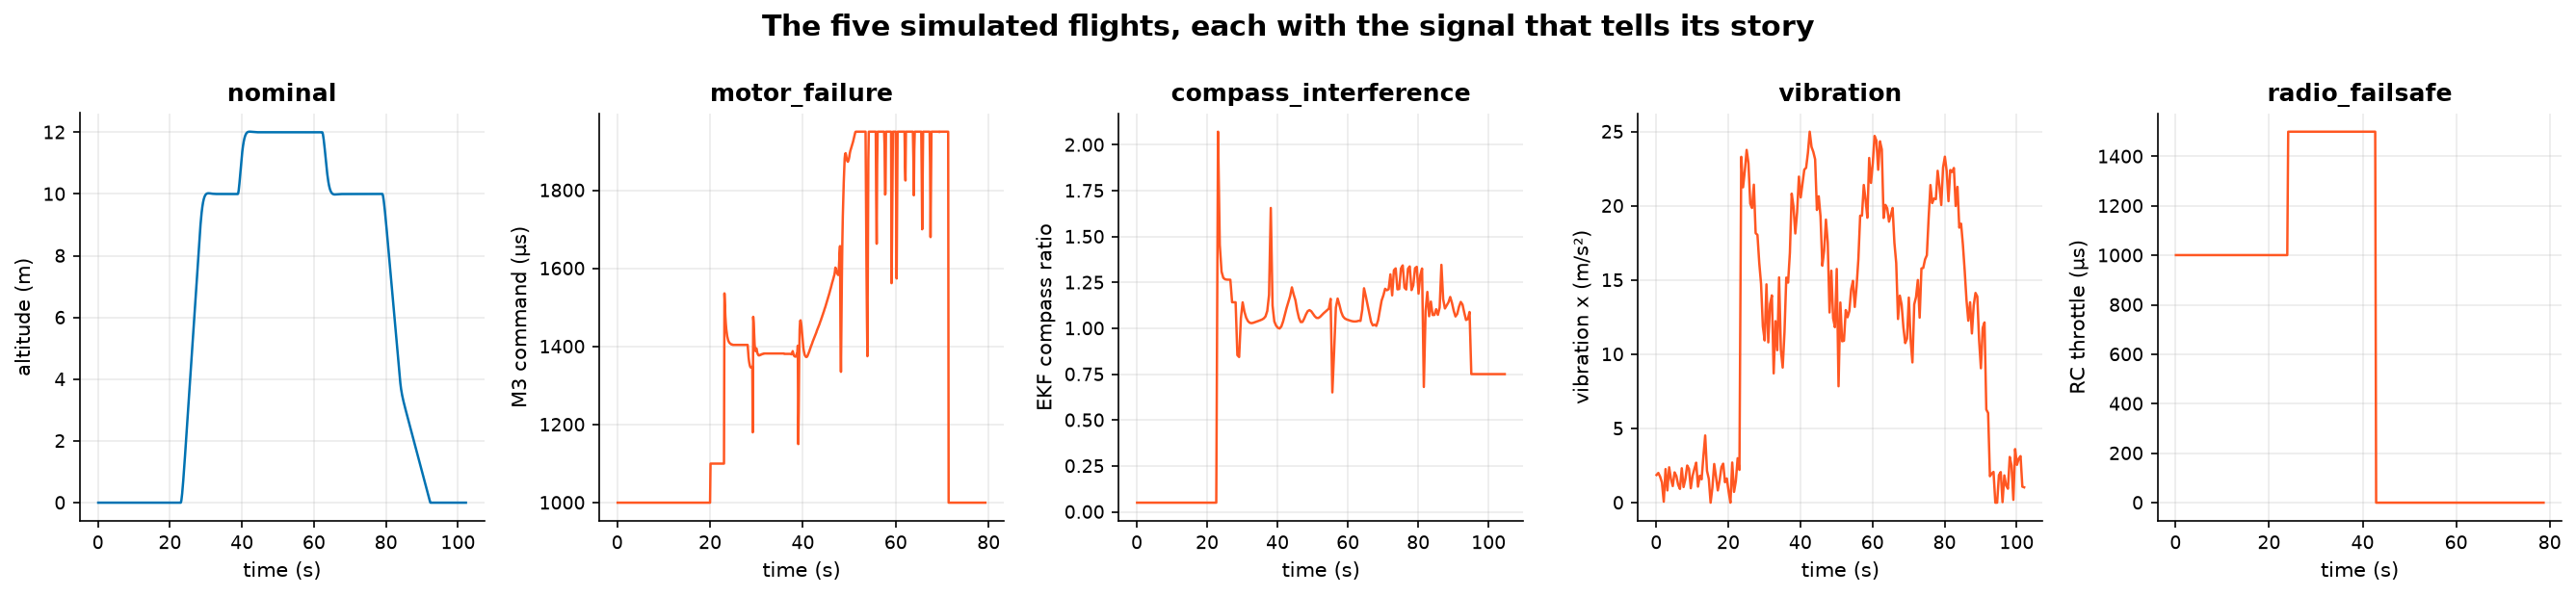
\includegraphics[width=\linewidth,height=0.42\textheight,keepaspectratio]{images/guide/30_scenarios_overview.png}
\caption{Scenarios overview}
\end{figure}

\begin{center}\small
\begin{tabularx}{\linewidth}{XXX}
\toprule
Scenario & What is injected & What AnaTele finds \\
\midrule
\texttt{nominal} & nothing & only the configuration note \texttt{fs-gcs-disabled} \\
\texttt{motor\_\allowbreak{}failure} & motor 3 health $\max(0.3, 1 - 0.06(t - t_f))$ from 2 s after WP3 becomes active & tracking loss, ceiling saturation, imbalance; \emph{thrust/configuration: strong support} \\
\texttt{compass\_\allowbreak{}interference} & heading error that grows with motor current & EKF compass innovation above 1 for 24.5 s \\
\texttt{vibration} & random torque noise (a damaged prop) & persistent vibration, 283 clips \\
\texttt{radio\_\allowbreak{}failsafe} & RC signal lost mid-mission & pre-arm \emph{radio failsafe} reports \\
\bottomrule
\end{tabularx}
\end{center}

\begin{guidebox}{Make your own}{green!40!black}
\texttt{Simulator(scenario, seed, mission=[...], wind=(n, e))} in \texttt{telemetry\_\allowbreak{}platform/simulator.py} takes your own
mission and wind. Different seeds give different noise but the same physics.

\end{guidebox}
\begin{guidebox}{Careful}{orange!80!black}
The simulator is a teaching and testing model, not a certified flight dynamics model. Real crashes are messier.
Use it to understand the method, not to calibrate thresholds for a real aircraft.
\end{guidebox}
\chapter{Sharing with .ant files}
\label{ch:12-sharing-ant}

An investigation is often a team effort. The pilot, the builder and a reviewer may all need to see the same thing.
Instead of sending a raw log and hoping everyone uses the same version of every tool, AnaTele saves the **whole
analysis** as one file: \texttt{.ant}.

\begin{figure}[H]\centering
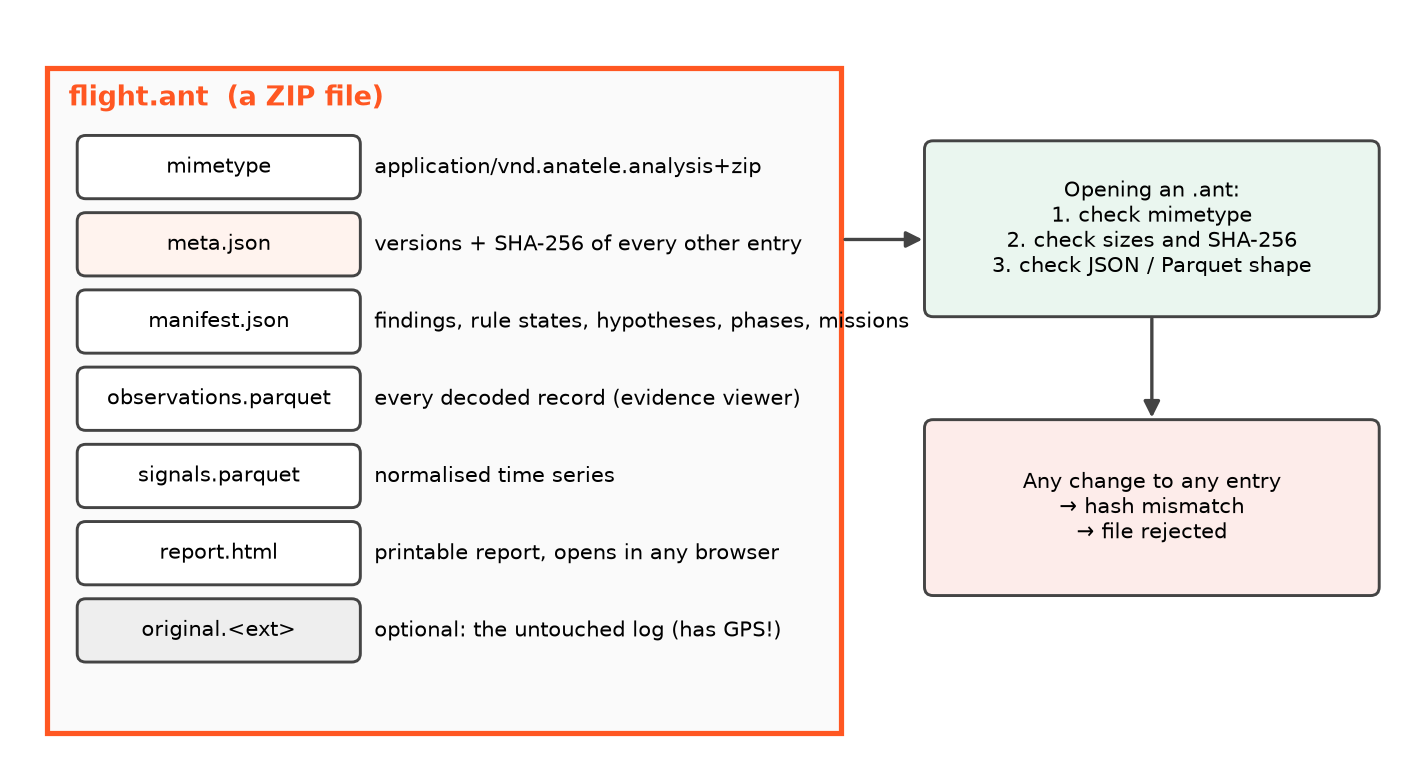
\includegraphics[width=\linewidth,height=0.42\textheight,keepaspectratio]{images/guide/31_ant_file.png}
\caption{.ant file}
\end{figure}

\section{What is inside}

An \texttt{.ant} is an ordinary ZIP file. You can open it with any unzip tool, but AnaTele checks it strictly:

\begin{enumerate}
\item \texttt{mimetype} must be exactly \texttt{application/vnd.anatele.analysis+zip}.
\item \texttt{meta.json} lists the \textbf{SHA-256} hash of every other entry. A SHA-256 hash is a 64-character fingerprint:
change one byte of a file and the fingerprint changes completely.
\item Each entry is size-limited, hashed and compared. The JSON and Parquet structure is validated \textbf{before}
anything is shown.
\end{enumerate}

Any mismatch and the file is rejected. A modified analysis can't pass as the original.

\section{Saving and opening}

\paragraph{Desktop}
\textbf{File $\rightarrow$ Save Analysis As (.ant)} (Ctrl+S). Open with \textbf{File $\rightarrow$ Open} or drag and drop.

\paragraph{Command line}
\begin{verbatim}
anatele export flight.tlog -o flight.ant            # analysis only
anatele export flight.tlog -o flight.ant --include-original
anatele analyse flight.ant                           # print the summary
\end{verbatim}

\paragraph{Web / API}
\texttt{GET /api/logs/\{id\}/export.ant} to download, \texttt{POST /api/analyses} to import.

\begin{guidebox}{Privacy}{orange!80!black}
\texttt{--include-original} embeds the untouched log, and that contains \textbf{GPS positions} (where you fly, often where
you live). Leave it out unless the receiver needs to re-run the analysis or inspect raw bytes.

\end{guidebox}
\section{The report inside}

\texttt{report.html} is a self-contained, printable report: findings, hypotheses, rule states, phases and the mission
table. It opens in any browser, so someone without AnaTele can still read the result.

\medskip\hrule\medskip

\textbf{You've finished the course.} Next: open a real log in the desktop app, use the
\href{https://avinashistoocool.github.io/AnaTele/USAGE/}{Usage guide} for the controls and the \href{https://avinashistoocool.github.io/AnaTele/DIAGNOSTICS/}{Diagnostics reference} for every rule.
\appendix
\chapter{Glossary}

\begin{center}\small
\begin{tabularx}{\linewidth}{p{0.30\linewidth}X}
\toprule
Term & Meaning \\
\midrule
\textbf{ArduPilot} & Open-source autopilot firmware for drones, planes, rovers and boats. \\
\textbf{Armed} & Motors are allowed to spin. An \emph{episode} is one armed period. \\
\textbf{Attitude} & Orientation of the drone: roll, pitch and yaw. \\
\textbf{Baseline altitude} & Median altitude over the first 2 s after arming, treated as ``ground''. \\
\textbf{Ceiling / floor} & The highest / lowest motor command allowed (\texttt{MOT\_\allowbreak{}SPIN\_\allowbreak{}MAX} / \texttt{MOT\_\allowbreak{}SPIN\_\allowbreak{}MIN}). \\
\textbf{Clipping} & An accelerometer reading hit the sensor's maximum, so the true value is unknown. \\
\textbf{DataFlash log} & On-board log (\texttt{.bin}/\texttt{.log}) written to the flight controller's SD card. \\
\textbf{EKF} & Extended Kalman Filter, ArduPilot's sensor-fusion estimator. \\
\textbf{Epoch} & A stretch of a log in which the clock only moves forward (split at reboots). \\
\textbf{Event guard} & The pre-event window ends 3 s before an autopilot crash report. \\
\textbf{Family (evidence)} & A group of related rules; its contribution to a hypothesis is capped at 1.5. \\
\textbf{Haversine} & Formula for distance between two latitude/longitude points on a sphere. \\
\textbf{Hypothesis} & A possible explanation, scored by evidence for and against. Not a probability. \\
\textbf{Innovation / test ratio} & How far a sensor reading is from the EKF's prediction, scaled so 1.0 is the limit. \\
\textbf{MAVLink} & The message protocol between drones and ground stations. \\
\textbf{Mixer} & Turns throttle/roll/pitch/yaw demands into individual motor commands. \\
\textbf{Persistence} & A condition must hold continuously for a minimum time to count. \\
\textbf{Pre-event window} & From takeoff to just before the upset or crash report; where rules look for causes. \\
\textbf{PWM} & Pulse width (\textmu{}s) sent to a motor controller; here 1000 = off, 2000 = full. \\
\textbf{Rule pack} & The versioned YAML file of all rules and hypotheses. \\
\textbf{Rule state} & triggered / not triggered / unassessable / not applicable. \\
\textbf{Saturation} & A motor stuck at its ceiling or floor, so the controller has no headroom left. \\
\textbf{Source} & One MAVLink sender (system id : component id), e.g. \texttt{1:1}. \\
\textbf{STATUSTEXT} & Human-readable text messages from the autopilot (e.g. ``Crash: Disarming''). \\
\textbf{Tilt error} & Angle between desired and actual thrust direction. \\
\textbf{.tlog} & Telemetry log saved by the ground station from the radio link. \\
\textbf{.ant} & AnaTele's shareable, hash-verified analysis file. \\
\textbf{Unassessable} & The data needed to check something is missing or too sparse. Never ``healthy''. \\
\textbf{WP\_RADIUS\_M} & How close the drone must get for a waypoint to count as reached. \\
\bottomrule
\end{tabularx}
\end{center}
\end{document}
